\documentclass[mathpazo]{cicp}

%\journal{Applied Mathematics and Computation}
\usepackage{graphicx}
\usepackage{amssymb}
\usepackage{amsmath}
\usepackage{amsthm}
\usepackage{amssymb}
\usepackage{amsfonts}
\usepackage{amsrefs}
%\usepackage{subfig}

\begin{document}

%\title{\emph{hp}-Finite Element Model of Poisson and Nernst-Planck\\ System of Equations}
\title{Modeling Ionic Polymer-Metal Composites\\ with Space-Time Adaptive Multimesh \emph{hp}-FEM}


\author[Deivid Pugal et.~al.]{Deivid Pugal\affil{1}\comma\affil{4},
Pavel Solin\affil{2}\comma\affil{3}\comma\corrauth,
Kwang J. Kim\affil{1}, and Alvo Aabloo\affil{4}}

\address{\affilnum{1}\ Mechanical Engineering Department, University of Nevada, Reno, NV, U.S.A.\\
\affilnum{2}\ Department of Mathematics and Statistics, University of Nevada, Reno, NV, U.S.A.\\
\affilnum{3}\ Institute of Thermomechanics, Prague, Czech Republic\\
\affilnum{4}\ Institute of Technology, Tartu University, Estonia}

\emails{{\tt david.pugal@gmail.com} (D.~Pugal), {\tt solin@unr.edu} (P.~Solin),
	{\tt kwangkim@unr.edu} (K.~Kim), {\tt alvo@ut.ee} (A.~Aabloo)}

%\author[unrme,tartu]{D.~Pugal}
%\ead{david.pugal@gmail.com}
%
%\author[unrmath,czech]{P.~Solin\corref{cor2}}
%\ead{solin@unr.edu}
%
%\author[unrme]{K.~J.~Kim\corref{cor1}}
%\ead{kwangkim@unr.edu}
%
%\author[tartu]{A.~Aabloo}
%\ead{alvo@ut.ee}
%
%\address[unrme]{Mechanical Engineering Department, University of Nevada, Reno, NV, U.S.A.}
%\address[unrmath]{Department of Mathematics and Statistics,
%University of Nevada, Reno, NV, U.S.A.}
%\address[czech]{Institute of Thermomechanics, Prague, Czech Republic}
%\address[tartu]{Institute of Technology, Tartu University, Estonia}
%
%\cortext[cor1]{Corresponding author}
%\cortext[cor2]{Principal corresponding author}

\begin{abstract}
We are concerned with a model of ionic polymer-metal composite (IPMC) materials
that consists of a coupled system of the Poisson and Nernst-Planck equations, 
discretized by means of the finite element method (FEM). We show that due to the 
transient character of the problem it is efficient to use adaptive algorithms 
that are capable of changing the mesh dynamically in time. We also show 
that due to large qualitative and quantitative differences between the 
two solution components, it is efficient to approximate them on different 
meshes using a novel adaptive multimesh \emph{hp}-FEM. The study is 
accompanied with numerous computations and comparisons of the adaptive 
multimesh \emph{hp}-FEM with several other adaptive FEM algorithms. 
\end{abstract}

%\begin{keyword}
%\keywords{Ionic polymer-metal composites, IPMC, Nernst-Planck equation, Poisson equation,
%finite element method, space-time adaptivity, multimesh \emph{hp}-FEM }
%\end{keyword}

%see http://www.ams.org/mathscinet/msc/msc2010.html?t=35Qxx&btn=Current

\ams{35Q84, 35Q05, 35J47}
\keywords{Ionic polymer-metal composites, IPMC, Nernst-Planck equation, Poisson equation,
finite element method, FEM, adaptive multimesh \emph{hp}-FEM }
\maketitle


%\end{frontmatter}

\section{Introduction}

Ionic Polymer-Metal Composites (IPMC) have been studied during the past two 
decades for their potential to serve as noiseless mechanoelectrical and electromechanical 
transducers \cite{basu1997membrane,shahinpoor2001smartmat,
nasser2002applied,newbury2003intelligent, wallmersperger2007appliedphysics,
pugal2008appliedphysics,pugal2010polymer}.
The advantages of IPMC over other electroactive polymer actuators
are low voltage bending, high strains ($>1\%$), and an ability to work
in wet environments. A typical IPMC consists of a thin sheet of polymer
(often Nafion or Teflon) which is sandwiched between noble
metal electrodes such as platinum or gold. When fabricated, the polymer 
membrane is saturated with certain solvent and ions such as water and $H^+$.
When a voltage is applied to the electrodes, the counter ions start
migrating due to the imposed electric field. By dragging along the solvent,
the osmotic pressure difference near the electrodes
results in bending of the material (see Fig.~\ref{fig:conceptual}).
\begin{figure}[!ht]
  \begin{centering}
  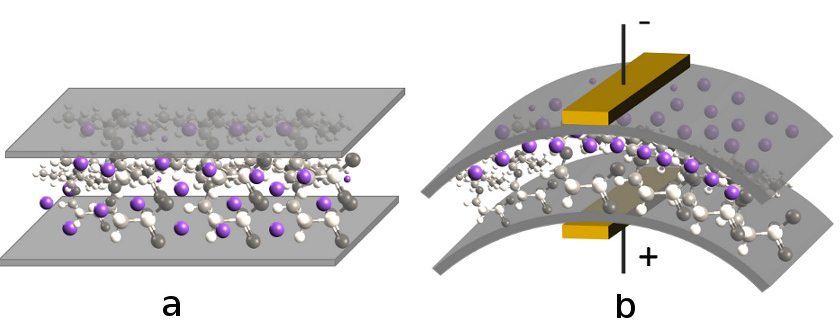
\includegraphics[scale=0.7]{IPMC_bending}
  \caption{\label{fig:conceptual}Conceptual model of the actuation
 	of IPMC. Initial counter ion distribution (a) and
	the distribution and resulting bending after applying a voltage (b).}
  \end{centering}
%\vspace{-1cm}
\end{figure}
%\newpage
%The derived and implemented model helps to predict the actuation of the
%material. Furthermore, it is expected that the \emph{hp}-FEM implementation
%results in a smaller problem size, thus likely allowing faster calculation
%in both 2D and 3D domains.

In this study we will model IPMC materials via a multiphysics coupled problem 
consisting of the Poisson and Nernst-Planck equations (abbreviated by PNP in
the following). These equations are used to model charge transport in materials 
that include ionic migration, diffusion, and convection. The charge transport 
process is a key mechanism for electromechanical transduction.

The PNP system is highly nonlinear and for a typical domain with two
electrodes, largest differences in charge concentration occur in a very narrow
region near the boundary. The computing power required for a full scale problem 
is significant~\cite{pugal2010spie3d}. This is why we are interested in exploring adaptive algorithms
-- we hope to obtain meshes that are optimal in terms of calculation time and 
calculation error.

The Nernst-Planck equation for a mobile species ---
in our case for counter ions --- has the form
\begin{equation}
  \frac{\partial C}{\partial t}+\nabla\cdot(-D\nabla C-\mu FC\nabla\phi)=0.
  \label{eq:nernst-planck}
\end{equation}
Here $C$ stands for the counter ion concentration, $D$ is diffusion, $\mu$ mobility,
$F$ Faraday constant, and $\phi$ voltage. We have neglected 
the velocity of the species as in our case it can be assumed zero. 
The Poisson equation has the form
\begin{equation}
  -\nabla^2\phi=\frac{F\rho}{\varepsilon}
  \label{eq:poisson}
\end{equation}
where $\varepsilon$ is the absolute dielectric permittivity. The
charge density $\rho = C-C_{0}$ 
where $C_{0}$ is a constant anion concentration.

The outline of the paper is as follows: Section \ref{sec:moti} shows that 
the solution components $C$ and $\phi$ have very different behavior, which
is the reason why it is difficult to find a common mesh that would be optimal 
for both of them. This explains why we are interested in approximation them
on individual meshes equipped with mutually independent adaptivity 
mechanisms. The PNP model is presented in Section \ref{sec:model} where also its weak 
formulation for the Newton's method is derived. Section \ref{sec:hermes}
presents a brief overview of a novel adaptive multimesh $hp$-FEM 
method~\cite{solin2010monolithic,solin2010adaptive,dubcova2010space,solini2010adaptive}
that is used to solve the 
problem numerically. Numerical results and comparisons are presented in Section 
\ref{sec:results}, and conclusion and outlook are drawn in Section \ref{sec:conc}.



\section{Motivation} \label{sec:moti}

In this section we use a simplified one-dimensional model to illustrate the 
principal difficulties encountered in the numerical solution of the 
PNP system.
Table~\ref{Table:used-constants} shows constants that we will use in 
computations in this section as well as in the rest of the paper: 

\begin{table}[!ht]
\caption{Constants used in the Poisson-Nernst-Planck system of equations.}
\centering
\label{Table:used-constants}
{
\begin{tabular}{llll}
  \hline \hline
  Constant&Value&Unit&Description\\
  \hline
  $D$&$10\times10^{-11}$&$\frac{m^2}{s}$&Diffusion constant\\
  $z$&1&-&Charge number\\
  $F$&96,485&$\frac{C}{mol}$&Faraday number\\
  $R$&8.31&$\frac{J}{mol\cdot K}$&The gas constant\\
  $\mu\ \left( = \frac{D}{RT}\right)$&$4.11\times 10^{-14}$&$\frac{s}{mol\cdot K}$&Mobility\\
  $C_{0}$&1,200&$\frac{mol}{m^3}$&Anion concentration\\
  $\varepsilon$&0.025&$\frac{F}{m}$&Electric permittivity\\
  \hline
  \hline
\end{tabular}
}
\end{table}


Fig.~\ref{fig:comsol-conc-volt} shows a typical solution for $C$ and $\phi$
at $t=0.1\ s$ and $t=3.0\ s$. 
The solution has 
two notable characteristics: For the most part of the domain $\Omega$,
the gradient $\nabla C = 0$. Close to $\partial \Omega_2$, $\nabla C$ is
nonzero and moving in time, and $\nabla C$ is very large at $\partial \Omega_1$.
At the same time, $\phi$ is a "nice" smooth function for the most part of 
$\Omega$ but it has a large gradient at $\partial \Omega_2$.
This makes the choice of an optimal mesh extremely difficult. Even if the 
solution was stationary, an optimal mesh for $C$ could never be 
optimal for $\phi$ and vice versa.


\begin{figure}[!ht]
  \begin{centering}
      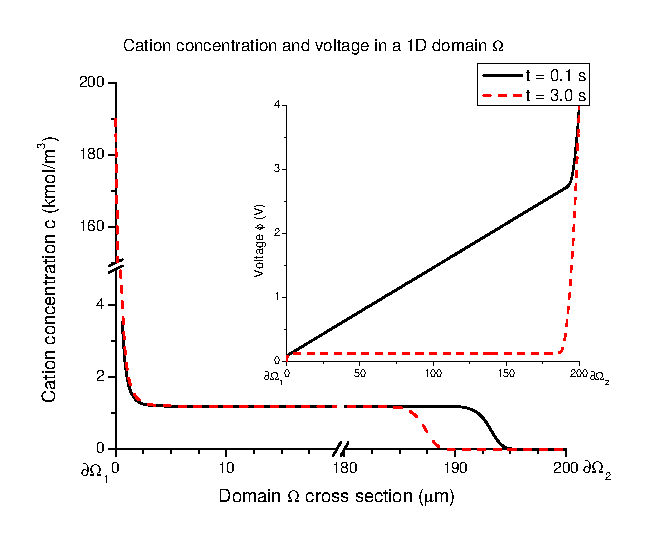
\includegraphics[]{comsol_conc_volt}
  \caption{Sample concentration $C$ and voltage $\phi$
           in a 1D domain $\Omega\subset\mathbb{R}$.
           Dirichlet boundary conditions ($V_{\partial \Omega_1}=0\ V$
           and $V_{\partial \Omega_2}=4\ V$) were
	   applied to the Poisson equation \eqref{eq:poisson} and Neumann conditions
	   to the Nernst-Planck equation \eqref{eq:nernst-planck}.}
\label{fig:comsol-conc-volt}
  \end{centering}
\end{figure}



Furthermore, the shape of the solution in Fig.~\ref{fig:comsol-conc-volt}
suggests that the polynomial degree of finite elements in the middle
of the domain $\Omega$ and near the boundaries $\partial \Omega_1,\ \partial \Omega_2$
should be different --- large high-degree elements should be used in the middle of the 
domain while small low-degree ones should be used in the boundary layers.  
The qualitative differences in the solution components $C$ and $\phi$ 
also suggest that using different meshes would be beneficial. 

% THIS DOES NOT BELONG HERE
%All the aforementioned concerns can be solved by using
%a time dependent adaptive multimesh \emph{hp}-FEM solver.
%Automatic time dependent adaptivity in conjuction with \emph{hp}-FEM 
%helps to limit the error of the calculations by automatically choosing
%a suitable mesh and polynomial degrees of the elements at each time step.
%In this work Hermes~\cite{Hermes-project} was used to implement
%the PNP system and study
%the problem size, error convergence and solution time 
%with different refinement modes.




\section{Model}
\label{sec:model}

\begin{figure}
  \begin{centering}
  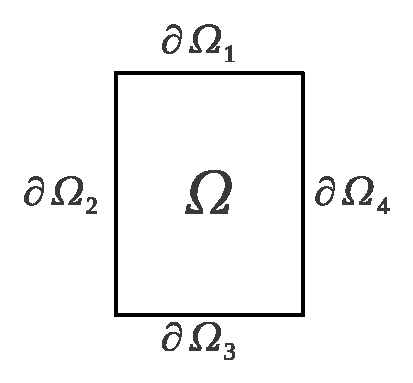
\includegraphics[width=0.2\columnwidth]{domain}
  \caption{\label{fig:domain} Calculation domain $\Omega\subset\mathbb{R}^2$
  	with boundaries $\partial\Omega_{1\ldots 4}\subset\partial\Omega$.}
  \end{centering}
\end{figure}

The model for solving PNP system is implemented in Hermes.
A rectangular 2D domain $\Omega\subset\mathbb{R}^2$ with boundaries 
$\partial\Omega_{1\ldots 4}\subset\partial\Omega$  is considered (see Fig.~\ref{fig:domain}). 
As there is no flow considered into or out from the domain and there is no
constant concentration at the boundaries, zero Neumann boundary conditions were used 
for Eq.~\eqref{eq:nernst-planck}:
\begin{equation}
  -D \frac{\partial C}{\partial n} - z \mu F C \frac{\partial \phi} {\partial n} = 0.
  \label{eq:nernst-planck-boundary}
\end{equation}
As a positive constant voltage $V_{pos}$ was applied on $\Omega_1$ and $V_{neg}=0$ was applied
on $\Omega_3$, Dirichlet boundary conditions were used for Eq.~\eqref{eq:poisson} for
boundaries $\Omega_1$ and $\Omega_3$:
\begin{eqnarray}
  \phi_{\partial\Omega_1}&=&V_{pos},\\
  \phi_{\partial\Omega_3}&=&0,
  \label{eq:dirichlet}
\end{eqnarray}
and Neumann boundaries for $\Omega_2$ and $\Omega_4$:
\begin{equation}
  \frac{\partial \phi_{\Omega_2}}{\partial n}=\frac{\partial \phi_{\Omega_4}}{\partial n}=0.
\end{equation}


\subsection{Weak form of Poisson-Nernst-Planck system}

The initial more implicit version of the derived weak form of PNP
was derived in~\cite{pugal2010spie}.
To make the derivation of the weak forms more convenient, the following
constants are used: 
\begin{eqnarray}
  K & = &z \mu F,\\
  L&=&\frac{F}{\varepsilon}.
  \label{eq:KL}
\end{eqnarray}
So Eq.~\eqref{eq:nernst-planck} and Eq.~\eqref{eq:poisson} become after 
substituting Eq.~\eqref{eq:rho} and the constants $K$ and $L$:
\begin{eqnarray}
  \frac{\partial C}{\partial t}-D\nabla^2 C-K\nabla\cdot \left(C\nabla\phi\right)&=&0,\label{eq:nernst-planck-2}\\
  -\nabla^2\phi-L\left(C-C_{0}\right)&=&0.\label{eq:poisson-2}
\end{eqnarray}
The boundary condition Eq.~\eqref{eq:nernst-planck-boundary} becomes:
\begin{equation}
  -D\frac{\partial C}{\partial n}-KC\frac{\partial\phi}{\partial n}=0.
  \label{eq:nernst-planck-boundary-2}
\end{equation}
The space for solution is $V=H^1\left(\Omega\right)$ where 
$H^1\left(\Omega\right)=\left\{v\in L^2\left(\Omega\right);\ \nabla v \in \left[L^2\left(\Omega\right)\right]^2\right\}$.
Let's choose a test function $v^C\in V$.
The weak form the Nernst-Planck equation Eq.~\eqref{eq:nernst-planck-2}
is found by multiplying it with the test function $v^C$ and then integrating over the domain~$\Omega$:
\begin{equation}
  \int_{\Omega}\frac{\partial C}{\partial t}v^C d\mathbf{x}
  -\int_{\Omega}D\nabla^2Cv^C d\mathbf{x}-\int_{\Omega}K\nabla C\cdot
  \nabla\phi v^C d\mathbf{x} - \int_{\Omega}KC\nabla^2\phi v^C d\mathbf{x}=0.
  \label{eq:nernst-planck-weak1}
\end{equation}
After adding the weak form of the boundary term 
(Eq.~\eqref{eq:nernst-planck-boundary-2}) and applying
the Green's first identity to the terms that contain Laplacian $\nabla^2$ we get
\begin{eqnarray}
 && \int_{\Omega}\frac{\partial C}{\partial t}v^C d\mathbf{x}+
  D\int_{\Omega}\nabla C\cdot\nabla v^C d\mathbf{x}-
  K\int_{\Omega}\nabla C \cdot \nabla \phi v^C d\mathbf{x}+
  K\int_{\Omega}\nabla\left(Cv^C\right)\cdot \nabla \phi d\mathbf{x}\\
  &&-D\int_{\partial\Omega}\frac{\partial C}{\partial n}v^C d\mathbf{S}-
  \int_{\partial\Omega}K\frac{\partial\phi}{\partial n}Cv^C d\mathbf{S}=0.
  \label{eq:nernst-planck-weak2}
\end{eqnarray}
After expanding the nonlinear term and given that the boundary terms
do not contribute, the weak form becomes
\begin{equation}
  \int_{\Omega}\frac{\partial C}{\partial t}v^C d\mathbf{x}+
  D\int_{\Omega}\nabla C \cdot \nabla v^C d\mathbf{x}-
  K\int_{\Omega}\nabla C \cdot \nabla \phi v^C d\mathbf{x}+
  K\int_{\Omega}\nabla \phi \cdot \nabla C v^C d\mathbf{x}+
  K\int_{\Omega} C \left(\nabla\phi\cdot\nabla v^C\right) d\mathbf{x}=0.
  \label{eq:nernst-planck-weak3}
\end{equation}
As the second and third term cancel out, the final weak from of 
the Nernst-Planck equation is
\begin{equation}
  \int_{\Omega}\frac{\partial C}{\partial t}v^C d\mathbf{x}+
  D\int_{\Omega}\nabla C \cdot \nabla v^C d\mathbf{x}+
  K\int_{\Omega} C \left(\nabla\phi\cdot\nabla v^C\right) d\mathbf{x}=0.
  \label{eq:nernst-planck-weak-final}
\end{equation}
Similarly the weak form of Poisson equation Eq.~\ref{eq:poisson-2}
with a test function $v^\phi\subset V$ is:
\begin{equation}
  -\int_{\Omega}\nabla^2\phi v^\phi d\mathbf{x}-\int_{\Omega}LCv^\phi d\mathbf{x}+
  \int_{\Omega}LC_{0}v^\phi d\mathbf{x}=0.
  \label{eq:poisson-weak1}
\end{equation}
After expanding the $\nabla^2$ terms, the final form becomes
\begin{equation}
  \int_{\Omega}\nabla\phi\cdot\nabla v^\phi d\mathbf{x}-\int_{\Omega}LCv^\phi d\mathbf{x}+
  \int_{\Omega}LC_{0}v^\phi d\mathbf{x}=0.
  \label{eq:poisson-weak-final}
\end{equation}


\subsection{Implementation in Hermes}
To implement the system of equations Eq.~\eqref{eq:nernst-planck-weak-final}
and Eq.~\eqref{eq:poisson-weak-final}, the residuals and the Jacobian
matrix were derived. For that, Crank-Nicolson time stepping was
used
\begin{equation}
  \frac{\partial C}{\partial t} \approx \frac{C^{n+1} - C^n}{\tau},
  \label{eq:cranic}
\end{equation}
where $\tau$ is a time step. For the variables $C^{n+1}$ and $\phi^{n+1}$ the
following notation will be used:
\begin{eqnarray}
  C^{n+1} &=& \sum_{k=1}^{N^C} y_k^{C} v_k^{C}, \label{eq:cnotation}j\\
  \phi^{n+1} &=& \sum_{k=1}^{N^{\phi}} y_k^{\phi} v_k^{\phi}\label{eq:phinotation},
\end{eqnarray}
where $v_k^C$ and $v_k^\phi$ are piecewise polynomial functions in $V$.
Considering the Crank-Nicolson time stepping and the notation~\eqref{eq:cnotation},
the time discretized Eq.~\eqref{eq:nernst-planck-weak-final} becomes
\begin{eqnarray}
  F_i^C\left(Y\right) & = & \int_{\Omega} \frac{C^{n+1}}{\tau}v_i^C d\mathbf{x} - 
  \int_{\Omega} \frac{C^{n}}{\tau}v_i^C d\mathbf{x}\nonumber\\
  &&+\frac 12 \left[D\int_{\Omega} \nabla C^{n+1} \cdot \nabla v_i^C d\mathbf{x}+ 
  	D\int_{\Omega} \nabla C^{n} \cdot \nabla v_i^C d\mathbf{x}\right]\nonumber\\
  &&+ \frac 12 \left[K\int_{\Omega}C^{n+1} \left(\nabla \phi^{n+1} \cdot \nabla v_i^C\right) d\mathbf{x}+
  K\int_{\Omega}C^{n} \left(\nabla \phi^{n} \cdot \nabla v_i^C\right) d\mathbf{x}\right]\label{eq:Fc},
\end{eqnarray}
and in the notation~\eqref{eq:phinotation}, Eq.~\eqref{eq:poisson-weak-final} becomes
\begin{equation}
  F_i^{\phi}\left(Y\right) = \int_{\Omega} \nabla \phi^{n+1} \cdot \nabla v_i^{\phi} d\mathbf{x} 
  - \int_{\Omega} LC^{n+1}v_i^{\phi} d\mathbf{x} + \int_{\Omega} LC_0 v_i^{\phi} d\mathbf{x}.
  \label{eq:Fphi}
\end{equation}
For the implementation the $2\times 2$ Jacobian matrix $DF/DY$ with elements corresponding to
\begin{equation}
  \frac{\partial F_i^C}{\partial y_j^C}, \ \frac{\partial F_i^C}{\partial y_j^{\phi}},\  
  \frac{\partial F_i^{\phi}}{\partial y_j^C}, \ \frac{\partial F_i^{\phi}}{\partial y_j^{\phi}},
\end{equation}
must be derived: 
\begin{eqnarray}
  \frac{\partial F_i^C}{\partial y_j^C} &=& 
  \int_{\Omega} \frac{1}{\tau} v_j^C v_i^C d\mathbf{x} + 
  \frac 12 D\int_{\Omega} \nabla v_j^C \cdot \nabla v_i^C d\mathbf{x}
  + \frac 12 K\int_{\Omega} v_j^C \left(\nabla \phi^{n+1} \cdot \nabla v_i^C\right) d\mathbf{x},\label{eq:dFcdyc}\\
  \frac{\partial F_i^C}{\partial y_j^{\phi}} &=&
  \frac 12 K \int_{\Omega} C^{n+1} \left(\nabla v_j^{\phi} \cdot \nabla v_i^C\right) d\mathbf{x},\\
  \frac{\partial F_i^{\phi}}{\partial y_j^C} &=&
  - \int_{\Omega} L v_j^C v_i^{\phi} d\mathbf{x},\\
  \frac{\partial F_i^{\phi}}{\partial y_j^{\phi}} &=&
  \int_{\Omega} \nabla v_j^{\phi} \cdot \nabla v_i^{\phi} d\mathbf{x}\label{eq:dFphidyphi}.
\end{eqnarray}
In Hermes Eq.~\eqref{eq:Fc} and \eqref{eq:Fphi} define the residuum $F$ and
Eq.~\eqref{eq:dFcdyc}---\eqref{eq:dFphidyphi} define the Jacobian matrix $J$.

\subsection{Adaptive multi-mesh solution in Hermes}

The defined Jacobian $J$ and residuum $F$ can be simply solved with Hermes by
using Newton's iteration. However, we were more interested in the automatic
adaptivity to control the error and problem size.

In a traditional low-order FEM, refining an element is not algorithmically complicated,
and so the most difficult part is to find out what elements should be refined. 
To do this, various techniques ranging from rigorous guaranteed a-posteriori 
error estimates to heuristic criteria such as residual error indicators, 
error indicators based on steep gradients, etc are employed. 
Unfortunately, none of these approaches are suitable for real-life 
multiphysics coupled problems or higher-order finite element methods: 
rigorous guaranteed error estimates only exist for very simple problems 
(such as linear elliptic PDE), and moreover only for low-order finite elements 
(such as piecewise linear approximations). These heuristic techniques 
are not employed in Hermes since they may fail 
in non-standard situations, and because they lack a 
transparent relation to the true approximation error.
In order to obtain fast, usable adaptivity, one has to resort to adaptive \emph{hp}-FEM.
Automatic adaptivity in the \emph{hp}-FEM is substantially different from adaptivity 
in low-order FEM, since every element can be refined in many different ways. 
Fig.~\ref{fig:refinements} shows several illustrative refinement candidates for a fourth-order element.
\begin{figure}
  \begin{centering}
  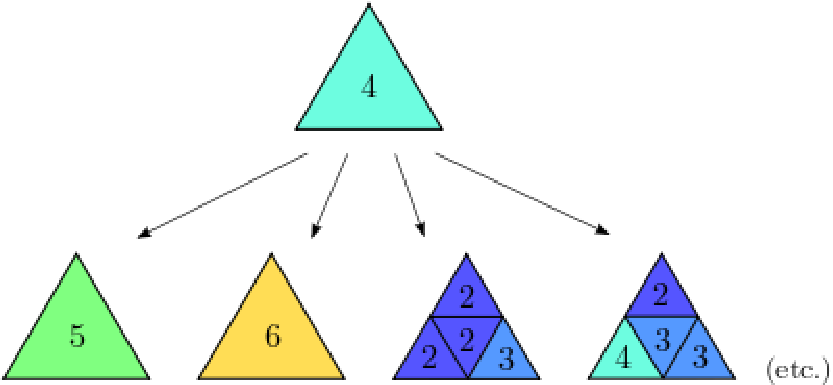
\includegraphics[width=0.5\columnwidth]{refinements}
  \caption{\label{fig:refinements} Refinement candidates for a fourth-order
  element.}
  \end{centering}
\end{figure}
The number of possible element refinements is implementation dependent. 
In general it is very low in \emph{h} or \emph{p} adaptivity, 
but much higher in \emph{hp}-adaptivity, and it rises even more when 
anisotropic refinements are enabled.
Hermes supports 8 different refinement modes, namely,
3 isotropic and 5 anisotropic refinements. The isotropic refinements are
\emph{h}-isotropic (H\_ISO), \emph{p}-isotropic (P\_ISO), \emph{hp}-isotropic (HP\_ISO).
Anisotropic refinement modes are
\emph{h}-anisotropic (H\_ANISO),
\emph{hp}-anisotropic-\emph{h} (HP\_ANISO\_H), \emph{p}-anisotropic (P\_ANISO),
\emph{hp}-anisotropic-p (HP\_ANISO\_P), and \emph{hp}-anisotropic (HP\_ANISO).
Due to the large number of refinement options, classical error estimators 
that provide a constant error estimate per element, cannot be used to 
guide automatic \emph{hp}-adaptivity. 
For this, one needs to know the shape of the approximation error.
Hermes uses a pair of approximations with different orders of accuracy 
to obtain this information: coarse mesh solution and fine mesh solution. 
The initial coarse mesh is read from the mesh file, and the initial 
fine mesh is created through its global refinement both in \emph{h}
and \emph{p}. The fine mesh solution is the approximation of 
interest both during the adaptive process and at the end of computation. 
The coarse mesh solution represents its low-order part.
Here global orthogonal projection of the fine mesh solution 
on the coarse mesh was used instead instead of solving on the coarse mesh.

\begin{figure}
  \begin{centering}
  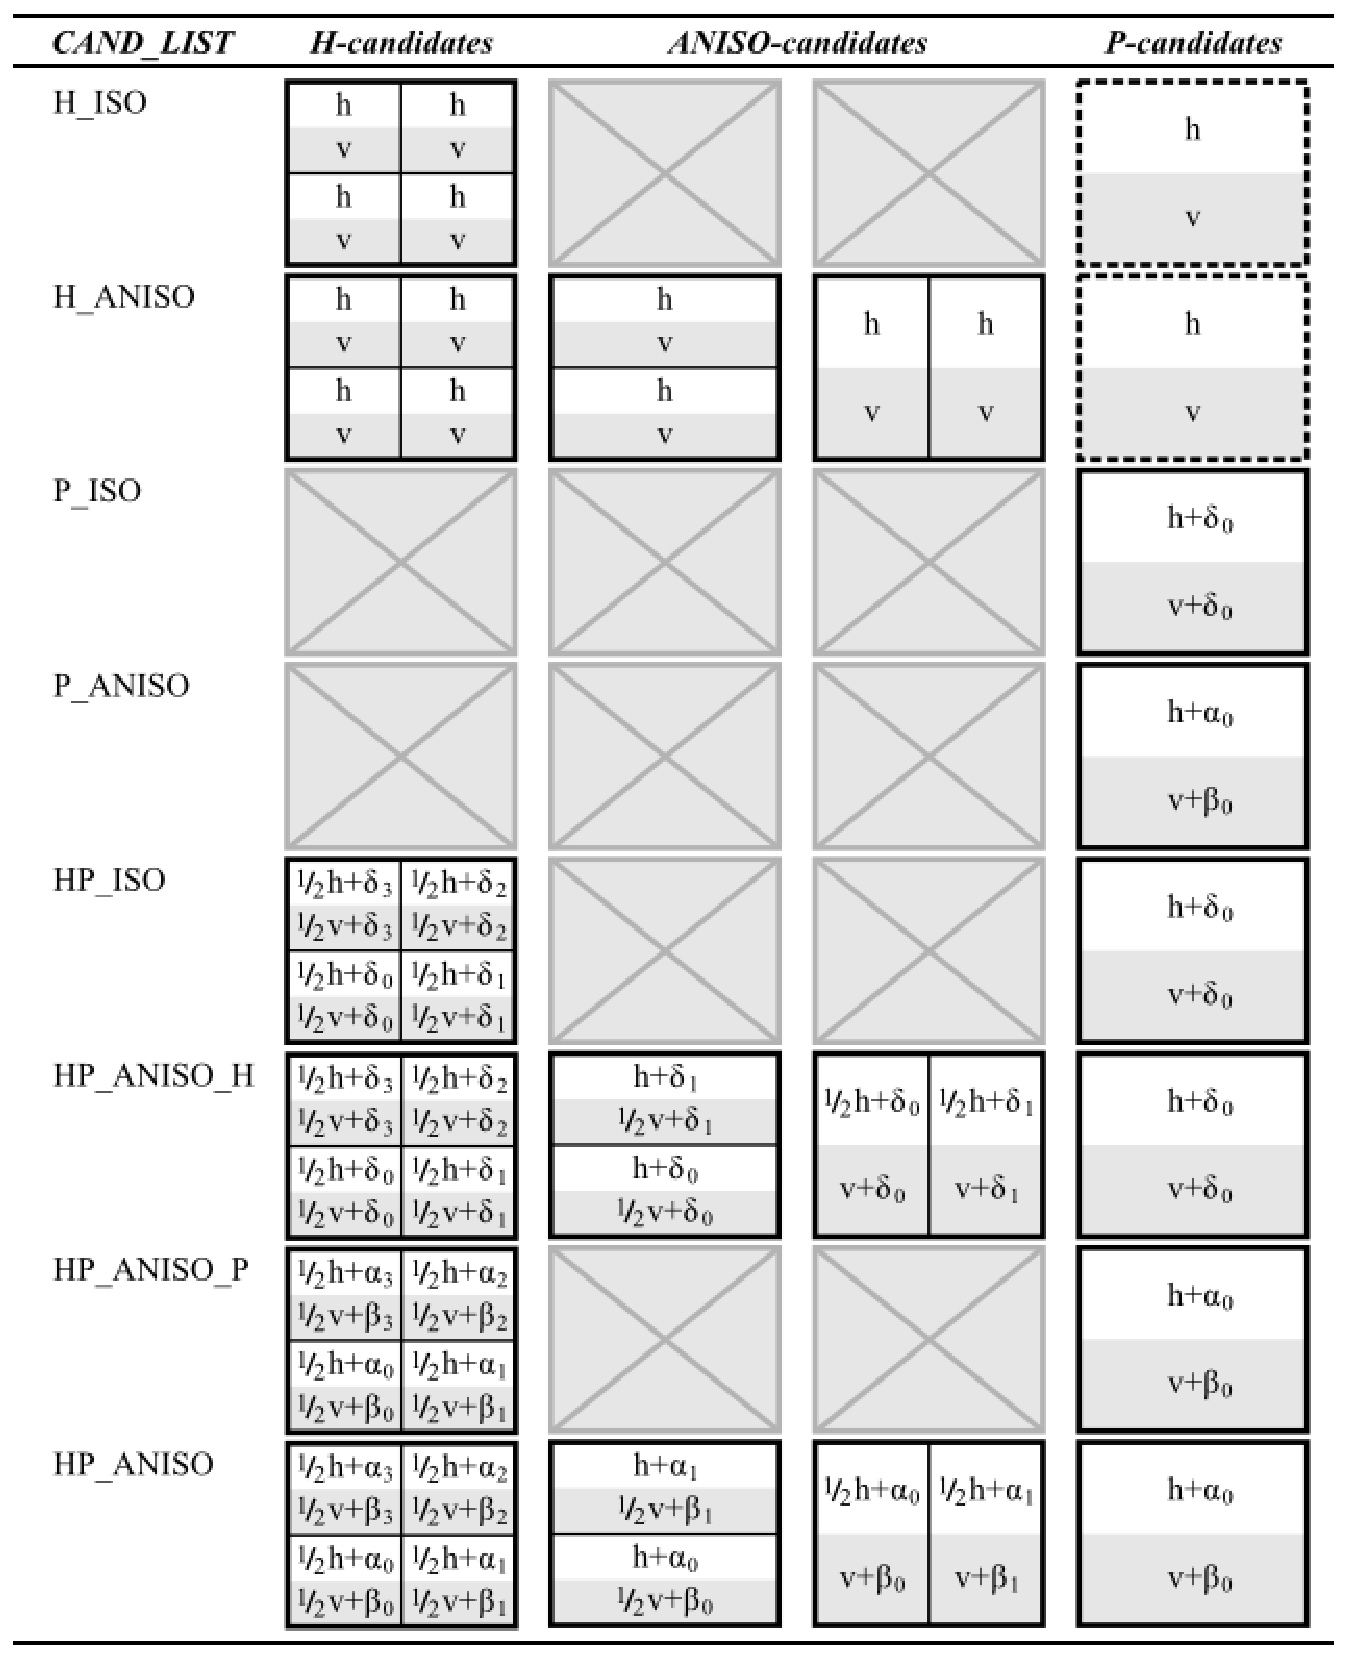
\includegraphics[width=0.5\columnwidth]{cand_list_quads}
  \caption{\label{fig:candlist} Refinement candidates for every
  refinement mode for quad type elements.}
  \end{centering}
\end{figure}
Refinement mode is selected by a user from among 8 modes listed before.
Hermes selects a particular
refinement scheme from several candidates based on the score which is
calculated as follows
\begin{equation}
	s=\frac{\log_{10} e_0 - \log_{10} e}{\left( d_0-d \right)^{\xi}},
\end{equation}
where $e$ and $d$ are an estimated error and an estimated
number of DOF of a candidate respectively, $e_0$ and $d_0$
are are an estimated error and an estimated number of DOF
of the examined element, respectively, and $\xi$ is a
convergence exponent. Here candidate
refers to a proposed refinement. Fig.~\ref{fig:candlist} shows all the proposed
refinements for all refinement modes in case of quad elements.
More information about the refinement modes and technical details
about the score calculation can be found in~\cite{Hermes-project}.

\begin{figure}
  \begin{centering}
  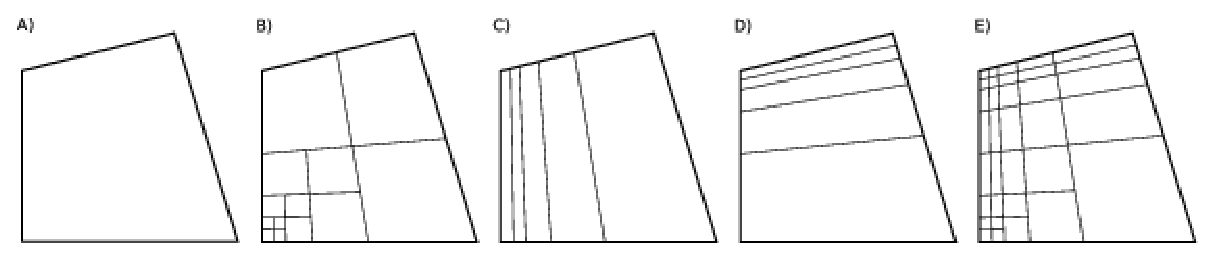
\includegraphics[width=0.5\columnwidth]{multimesh1}
  \caption{\label{fig:multimesh1} Master mesh (A) and 
  three different meshes for a coupled problem (B)~---~(D),
  and the virtual union mesh (E).}
  \end{centering}
\end{figure}
\begin{figure}
  \begin{centering}
  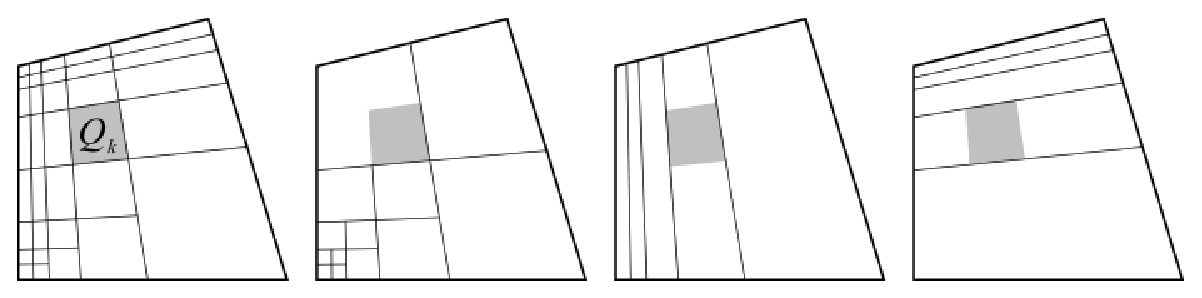
\includegraphics[width=0.5\columnwidth]{multimesh2}
  \caption{\label{fig:multimesh2} Integration over an element
  $Q_k$ of the virtual union mesh and the appropriate subelements
  of the existing elements where this integration is performed.}
  \end{centering}
\end{figure}
In multiphysics PDE systems such as Poisson-Nernst-Planck system it can 
happen that one physical field is very smooth whereas other one is not.
This is well shown in Fig.~\ref{fig:comsol-conc-volt}. 
If all the fields are approximated on the same mesh, then the necessity 
to refine the mesh at the steep gradient of a field implies new degrees 
of freedom for the smooth fields as well. This can be very wasteful.
Hermes makes it possible to approximate them on individual meshes. 
These meshes are not completely independent of each other --- they have 
a common coarse mesh that we call master mesh. The master mesh is 
there for algorithmic purposes only, it may not even be used for 
discretization purposes: Every mesh in the system is obtained from 
it via an arbitrary sequence of elementary refinements. 
This is illustrated in Fig.~\ref{fig:multimesh1}, where (A) is the master mesh, 
(B)~---~(D) three different meshes (say, for a coupled problem with three equations),
and (E) is the virtual union mesh that is used for assembling.
The union mesh is not constructed physically in the computer 
memory --- it merely serves as a hint to correctly transform  the 
integration points while integrating over sub-elements of an elements 
of the existing meshes. Fig.~\ref{fig:multimesh2} shows the integration
over an element $Q_k$ of the virtual union mesh.
As a result, the multimesh discretization of the PDE system is 
monolithic in the sense that no physics is lost --- all integrals 
in the discrete weak formulations are evaluated exactly up to 
the error in the numerical quadrature. 


\section{Numerical Results and Comparisons}\label{sec:results}


The solutions to the PNP problem exhibit a specific behavior that was 
described above. In order to find the best adaptive method to deal with 
this type of problems, we performed numerous computations using all 
adaptivity modes in both the single-mesh and multi-mesh regimes.
In the numerical experiments we paid attention to the 
relative error, cumulative CPU time, and problem size 
in terms of number of degrees of freedom (DOF) in each 
time step. The scaled variables $c$
and $\varphi$ and the unscaled time $t$ are used to present the solutions.
The simulations were performed with physical time step of $0.05$~s and
the final time of $3.0$~s was chosen as it is close to the time
scaling constant~$\tau$.  The time step was chosen after many
numerical experiments in such a way that the error
in time was approximately the same as the error in
space. The implementation of advanced adaptive
implicit higher-order Runge-Kutta methods is in progress.

We used two types of initial meshes --- a finer mesh shown 
in Fig.~\ref{fig:mesh}~(b) was used for \emph{p}-adaptivity
and a very coarse initial mesh shown in  Fig.~\ref{fig:mesh}~(a) was 
used for $h$-adaptivity and $hp$-adaptivity.

\begin{figure}[!ht]
  \begin{centering}
  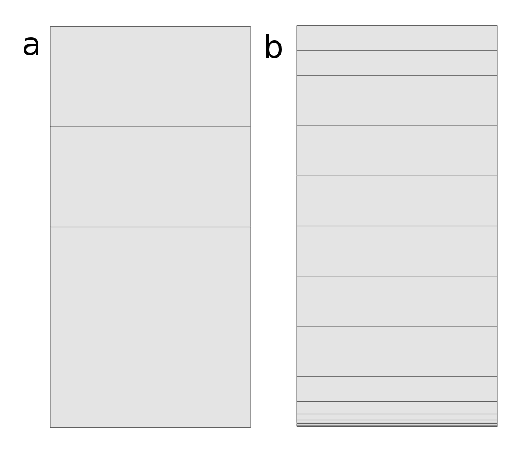
\includegraphics[width=.9\columnwidth]{mesh}
  \caption{\label{fig:mesh} Initial coarse mesh (a),
  	refined mesh (b), and symmetrically refined mesh for length scale study (c). 
	The coarse mesh (a)
	and refined mesh (b) were used in the initial calculations, the latter one
	in case of \emph{p}-adaptivity (including HP\_ANISO\_P).}
  \end{centering}
\end{figure}

An example of the solution at $t=0.1$~s and $t=3.0$~s
calculated with the HP\_ANISO refinement mode is shown
in Figs.~\ref{fig:cphi-1}~and~\ref{fig:cphi-2}. 

\begin{figure}[!ht]
  \begin{centering}
  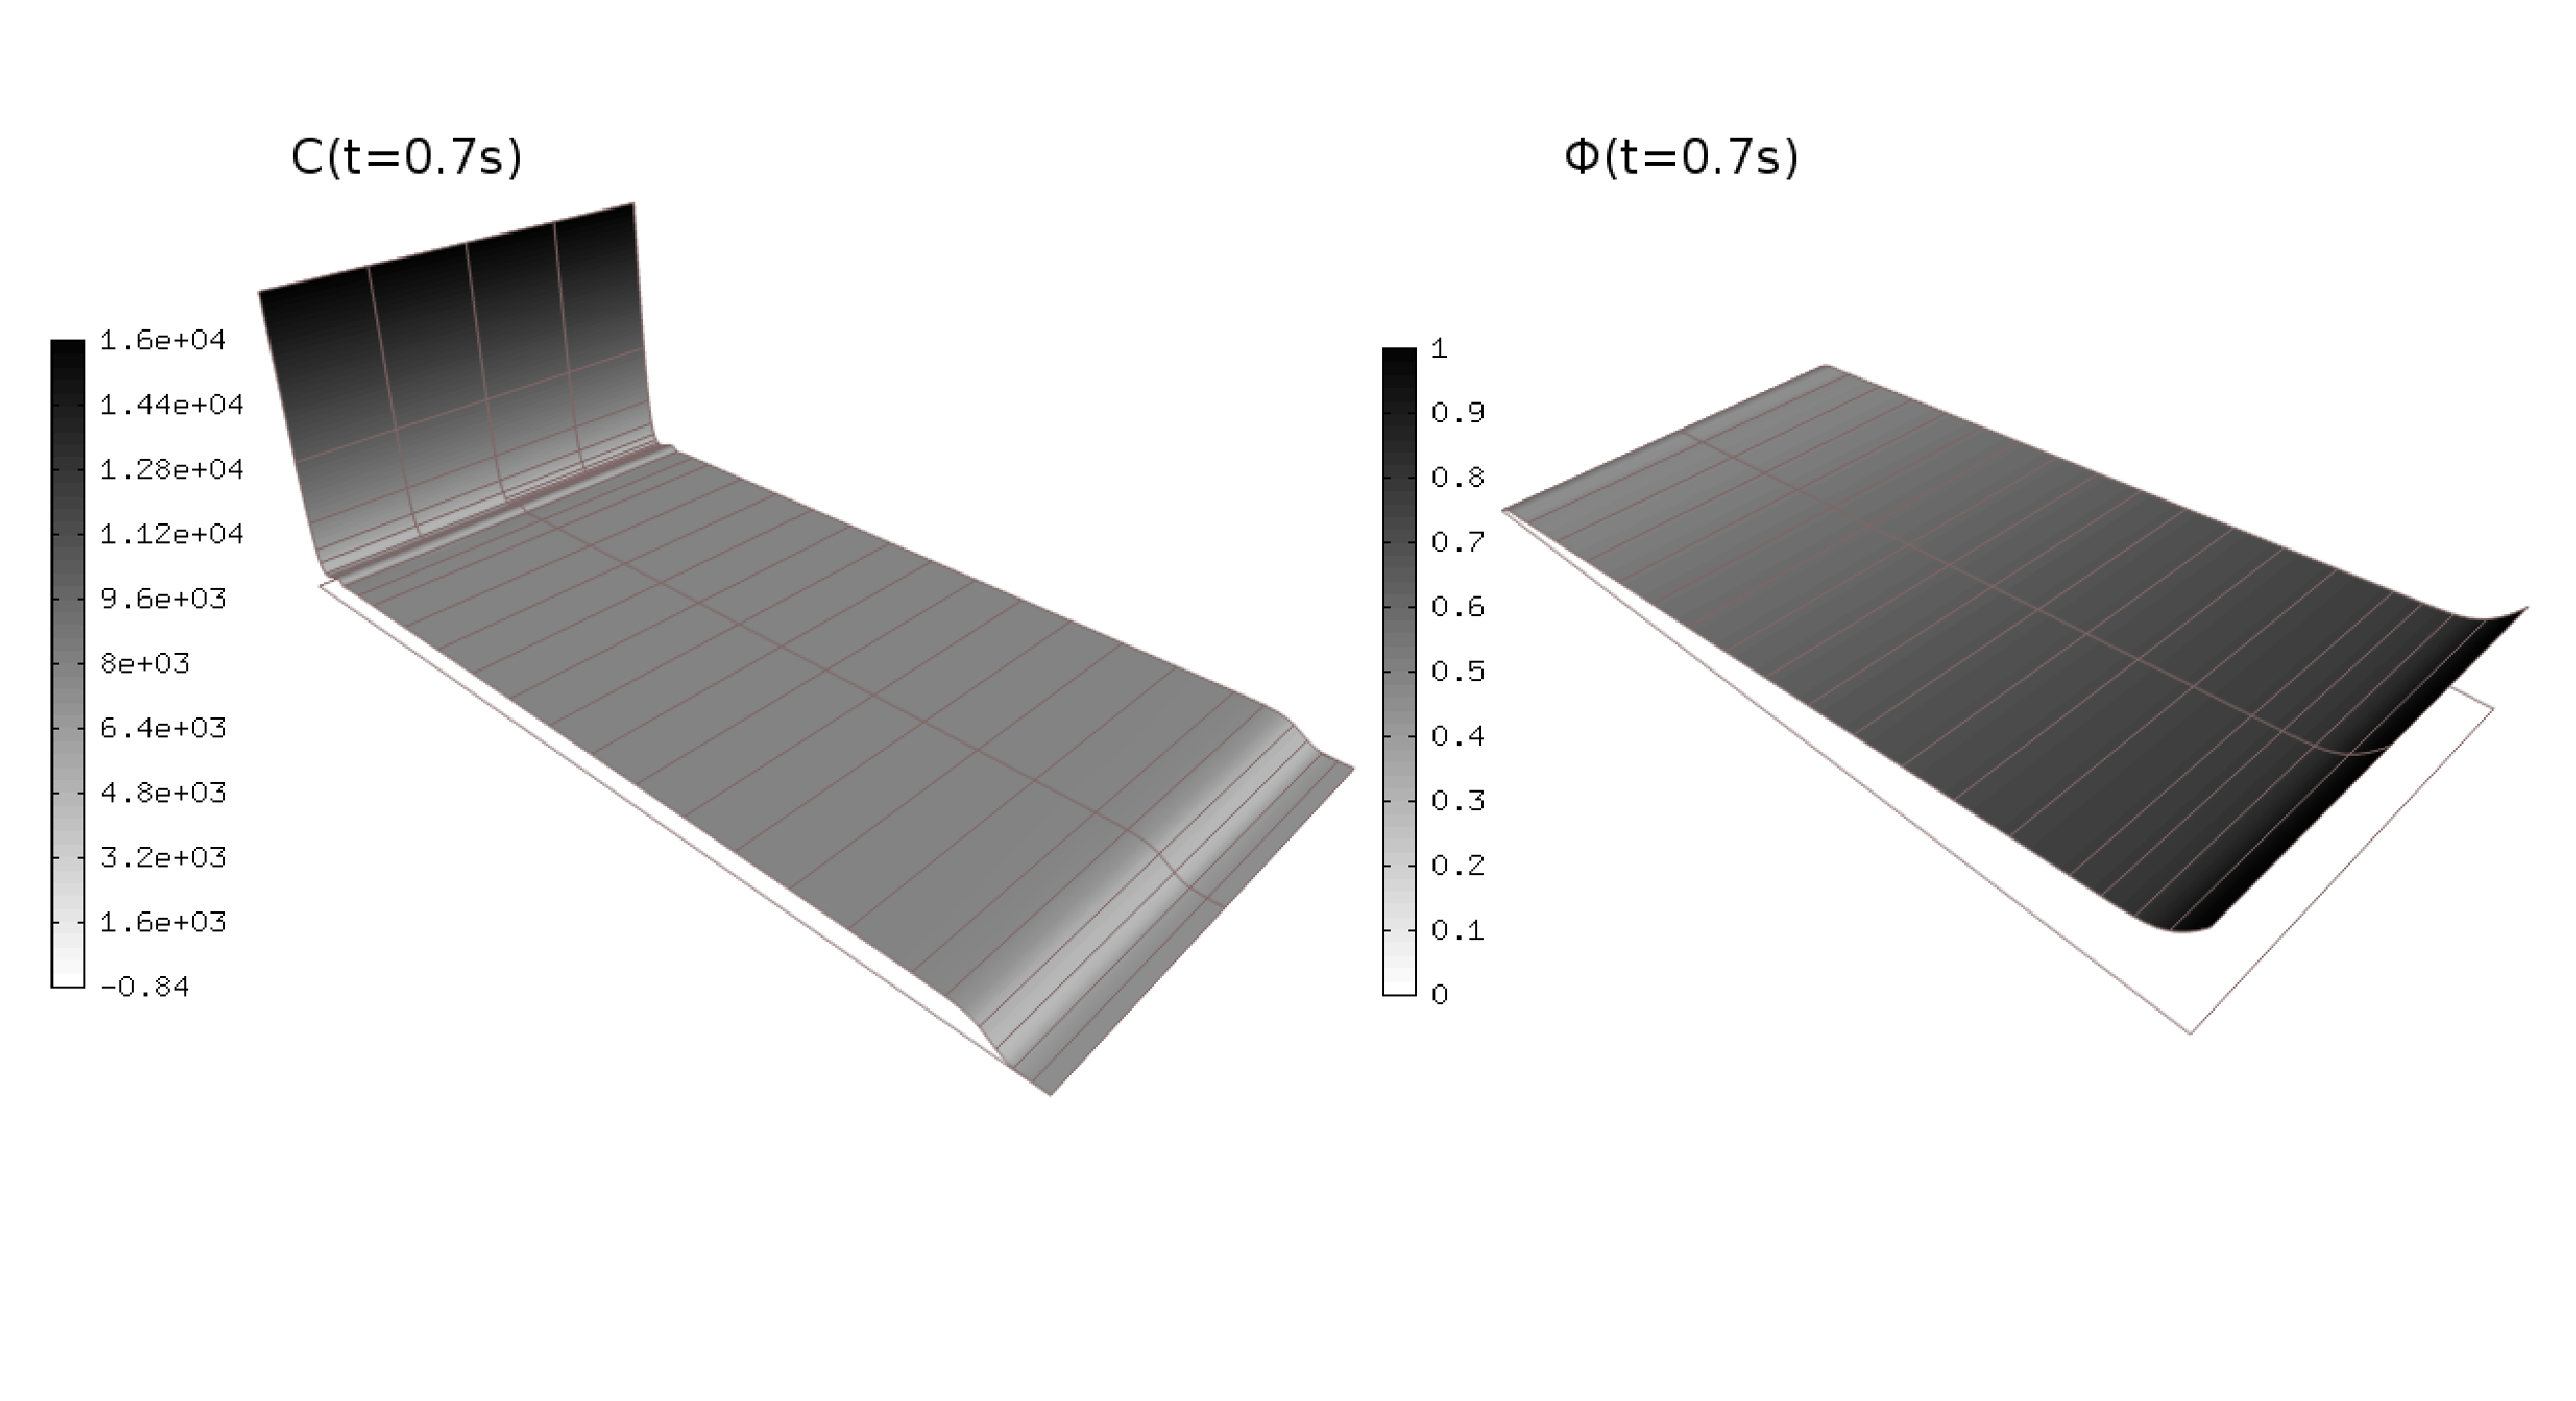
\includegraphics[width=\columnwidth]{cphi-1}
  \caption{\label{fig:cphi-1} Scaled concentration $c$
  and voltage $\varphi$ at $t=0.1\ s$.}
  \end{centering}
\end{figure}

\begin{figure}[!ht]
  \begin{centering}
  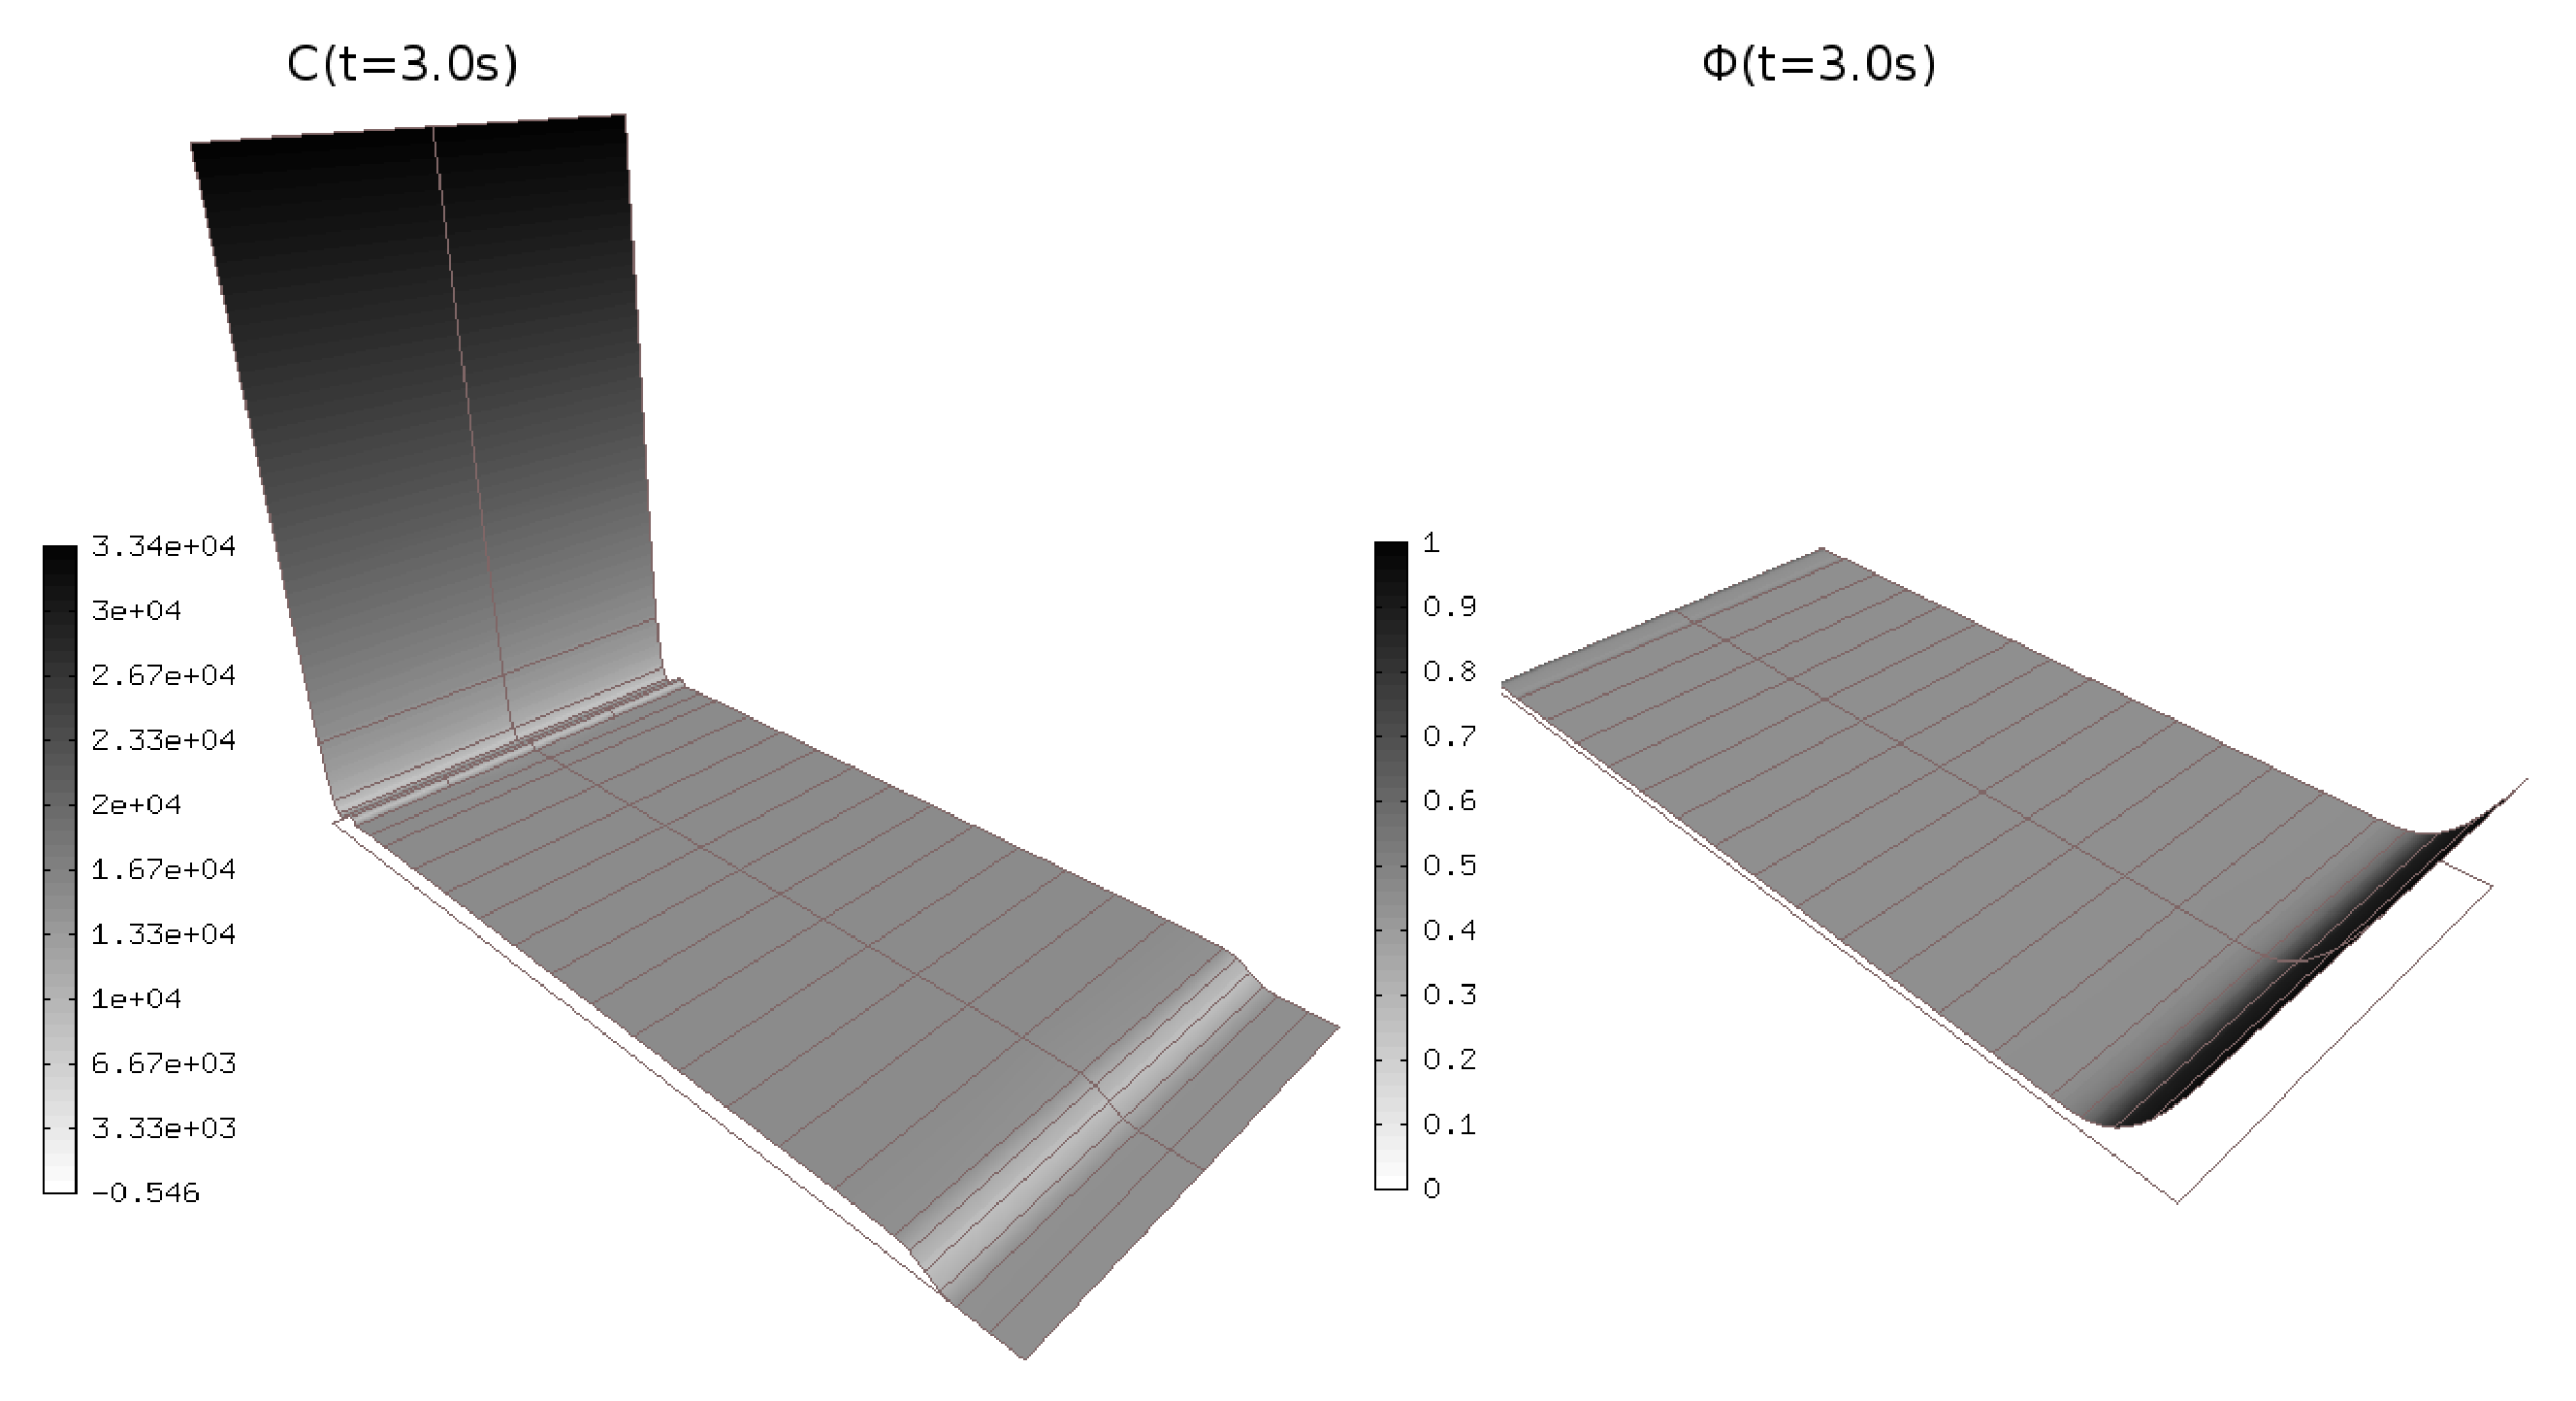
\includegraphics[width=\columnwidth]{cphi-2}
  \caption{\label{fig:cphi-2} Scaled concentration $c$
  and voltage $\varphi$ at $t=3.0\ s$.}
  \end{centering}
\end{figure}

The reader can see that at $t=0.1\ s$ some ionic migration has already 
taken place and large concentration gradients near the boundaries $\partial\Omega_1$ 
and $\partial\Omega_3$ have formed. The figures also show that the meshes 
at $t=0.1\ s$ and $t=3.0\ s$ are different. 

\subsection{Comparison of single mesh low-order FEM and $hp$-FEM}

First of all, the low-order FEM and $hp$-FEM were compared. A single mesh
H\_ANISO with polynomial degrees $p=1$ and $p=2$ were compared to
HP\_ANISO mode. The coarse initial mesh as shown in Fig.~\ref{fig:mesh}~(a)
was used in the solutions.
The results are shown in Figs.~\ref{fig:singlehhpdof} 
and~\ref{fig:singlehhpcpu}.
\begin{figure}[!ht]
  \begin{centering}
  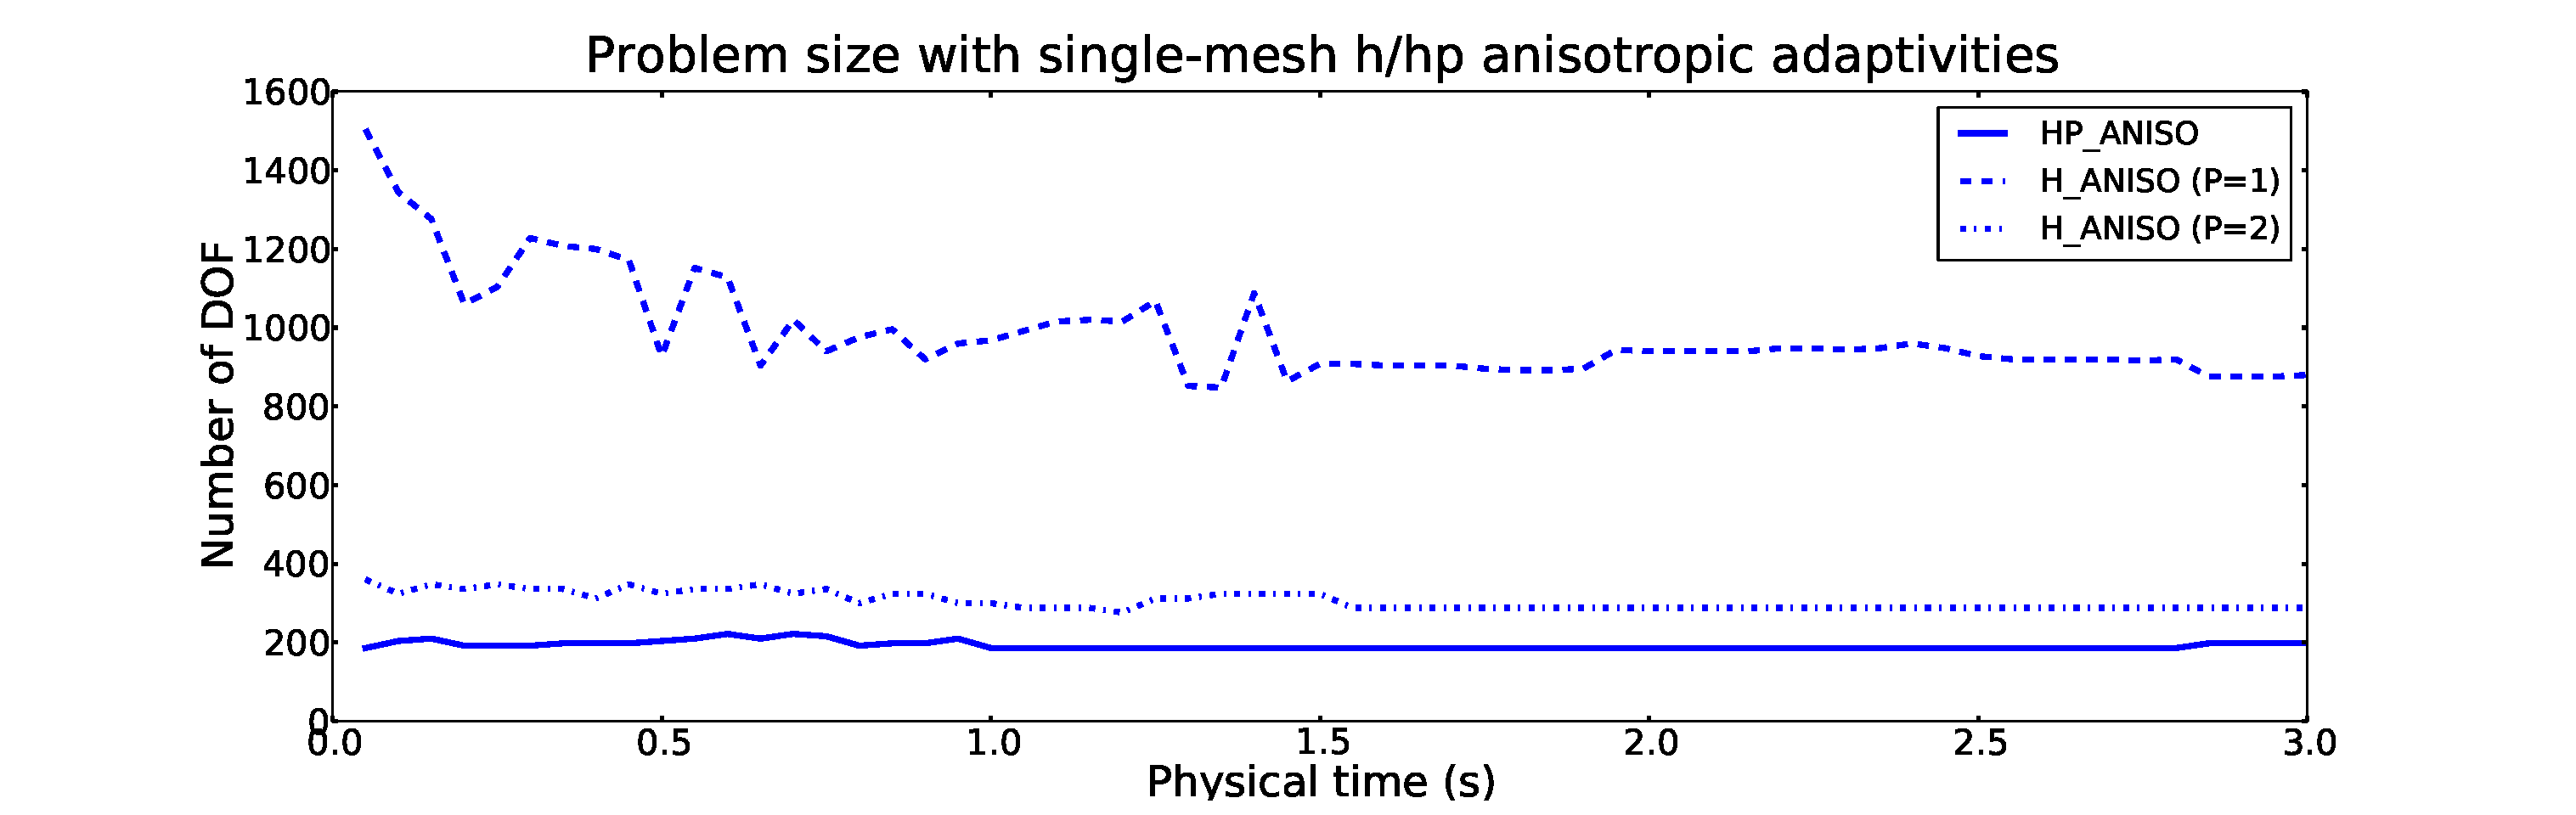
\includegraphics[width=\columnwidth]{singleh_hp_dof}
  \caption{\label{fig:singlehhpdof} Number of degrees of freedom (DOF) as a function 
  of physical time for single-mesh H\_ANISO (in case of
  $p=1$ and $p=2$) and single-mesh HP\_ANISO.}
  \end{centering}
\end{figure}


\begin{figure}[!ht]
  \begin{centering}
  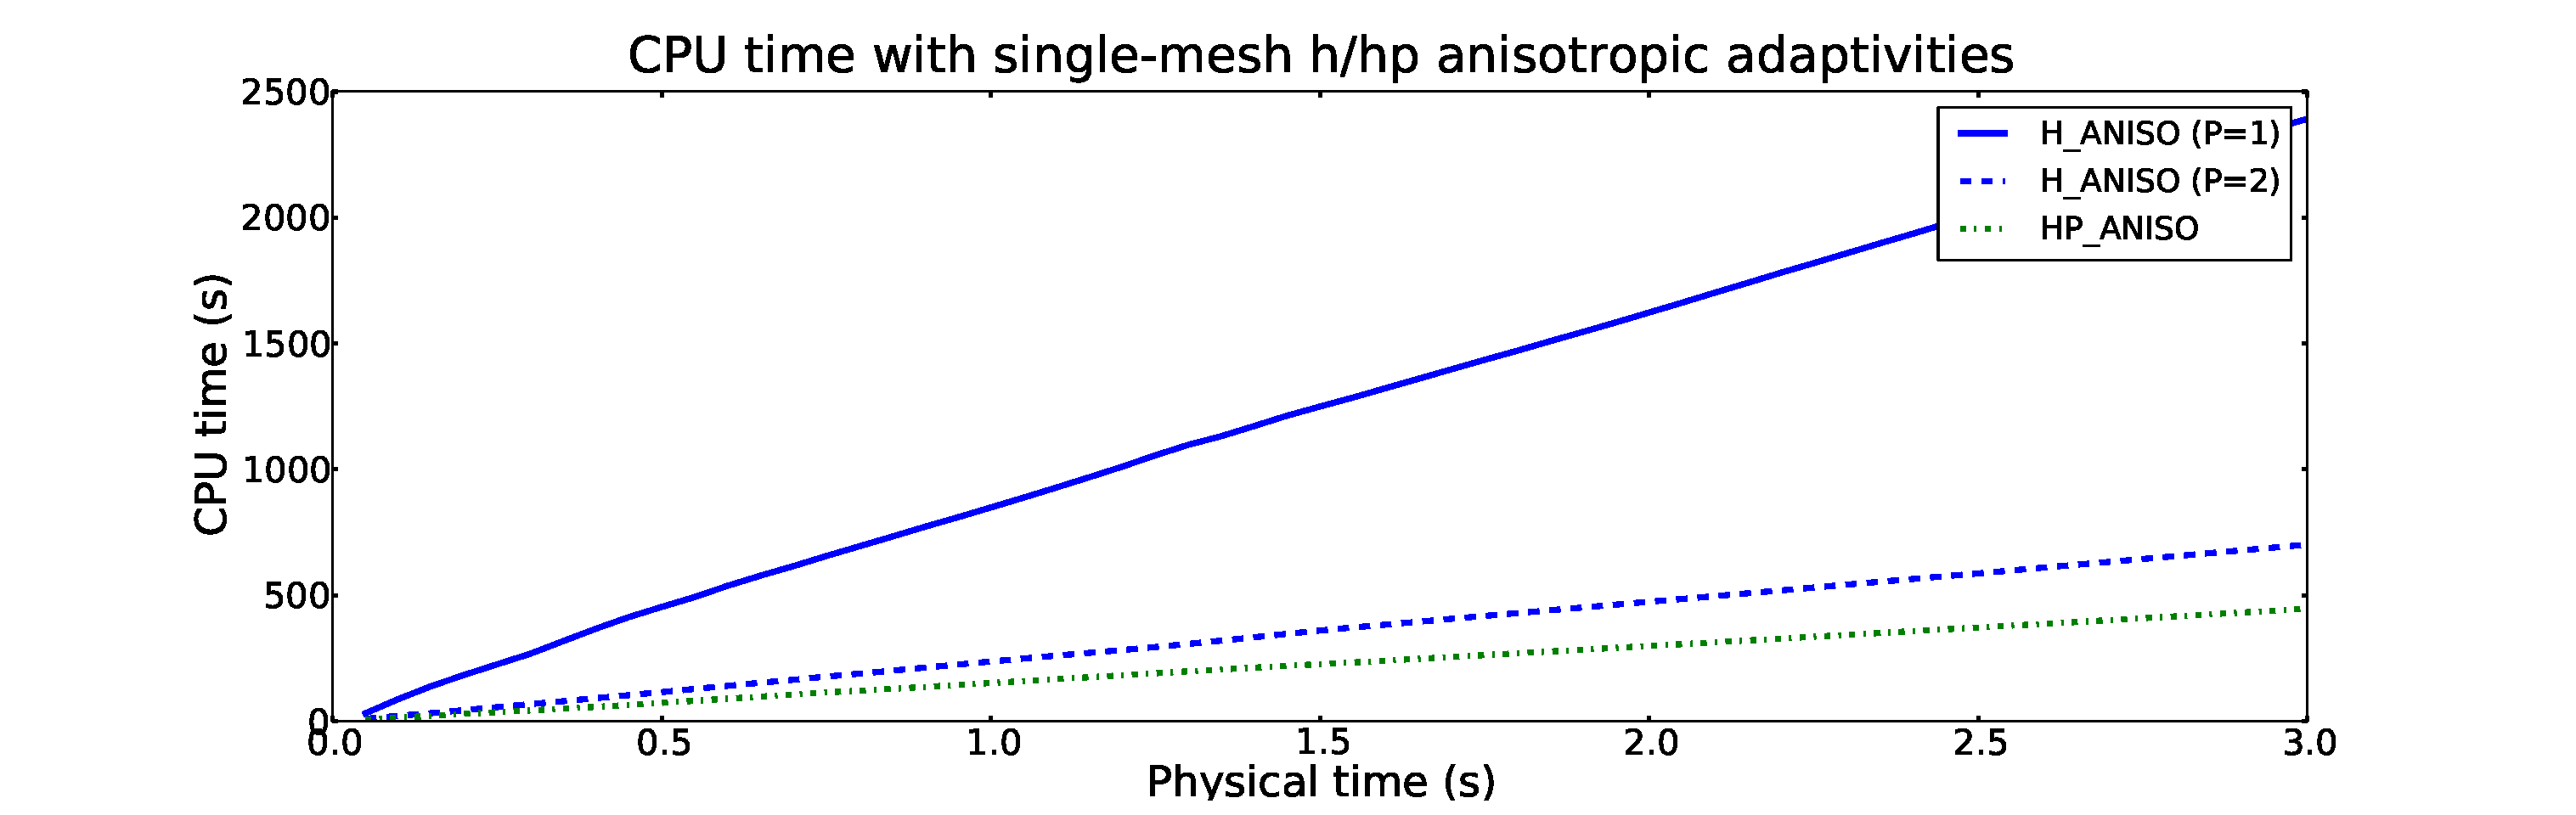
\includegraphics[width=\columnwidth]{singleh_hp_cpu}
  \caption{\label{fig:singlehhpcpu} Cumulative CPU time as a function 
  of physical time for single-mesh H\_ANISO (in case of $p=1$ and $p=2$)
  and single mesh HP\_ANISO.}
  \end{centering}
\end{figure}

\noindent
It can be seen that $hp$-FEM results in a shorter computing 
time and smaller number
of DOF than the low-order FEM. The same holds true
for H\_ISO and HP\_ISO modes. In fact, in case of H\_ISO the relative error did not
converge to the pre-set threshold value of $0.5\%$ within acceptable range 
of degrees of freedom of $nDOF_{threshold}=5000$.
Therefore, the $h$-FEM solutions will be omitted from the further comparisons.
Instead, only $hp$-FEM solutions on the coarse mesh and $p$-FEM solutions
on the fine mesh will be discussed.

\subsection{Comparison of single-mesh and multi-mesh $hp$-FEM}
Running the simulation with different adaptivity modes 
and meshes showed that the multi-mesh $hp$-FEM configuration resulted in
the smallest problems and similar error 
convergence compared to any single-mesh configuration. However,
multi-mesh problems generally resulted in longer computing times. This is a known
shortcoming of Hermes at this point and it is due to the fact that
multi-mesh uses the union mesh (see Section~\ref{sec:hermes}) where 
the numerical integration of high order is done on very small elements.
The problem size and computing time are illustrated for HP\_ANISO adaptivity mode in Fig.~\ref{fig:singlemultidof} and Fig.~\ref{fig:singlemulticpu}.
The same holds true for HP\_ISO mode.  It must be also noted that the error
converged to or below $0.5\%$ for all $p$-FEM and anisotropic $hp$-FEM results.
 
\begin{figure}[!ht]
  \begin{centering}
  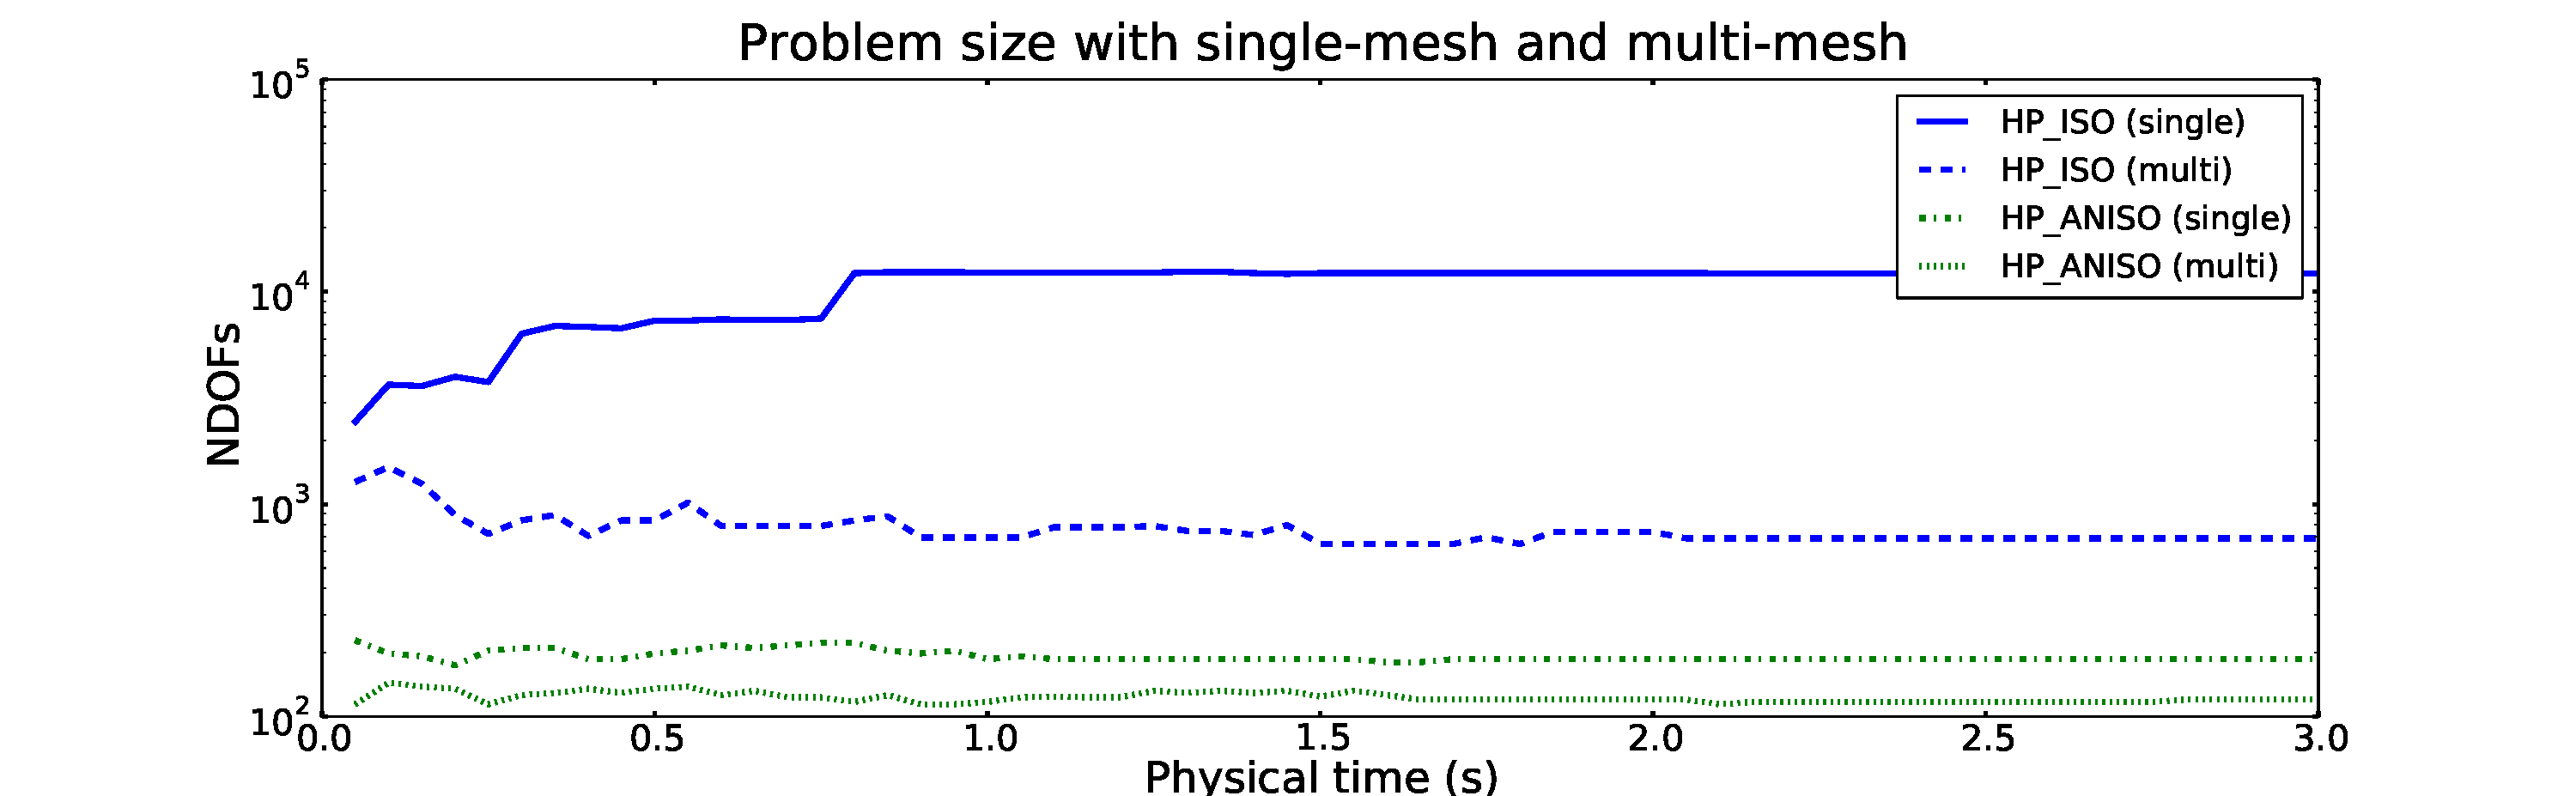
\includegraphics[width=\columnwidth]{singlemulti_dof}
  \caption{\label{fig:singlemultidof} Number of DOF as a function 
  of physical time for single-mesh and multi-mesh configurations with 
  HP\_ANISO adaptivity mode.}
%\vspace{-6mm}
  \end{centering}
\end{figure}


\begin{figure}[!ht]
  \begin{centering}
  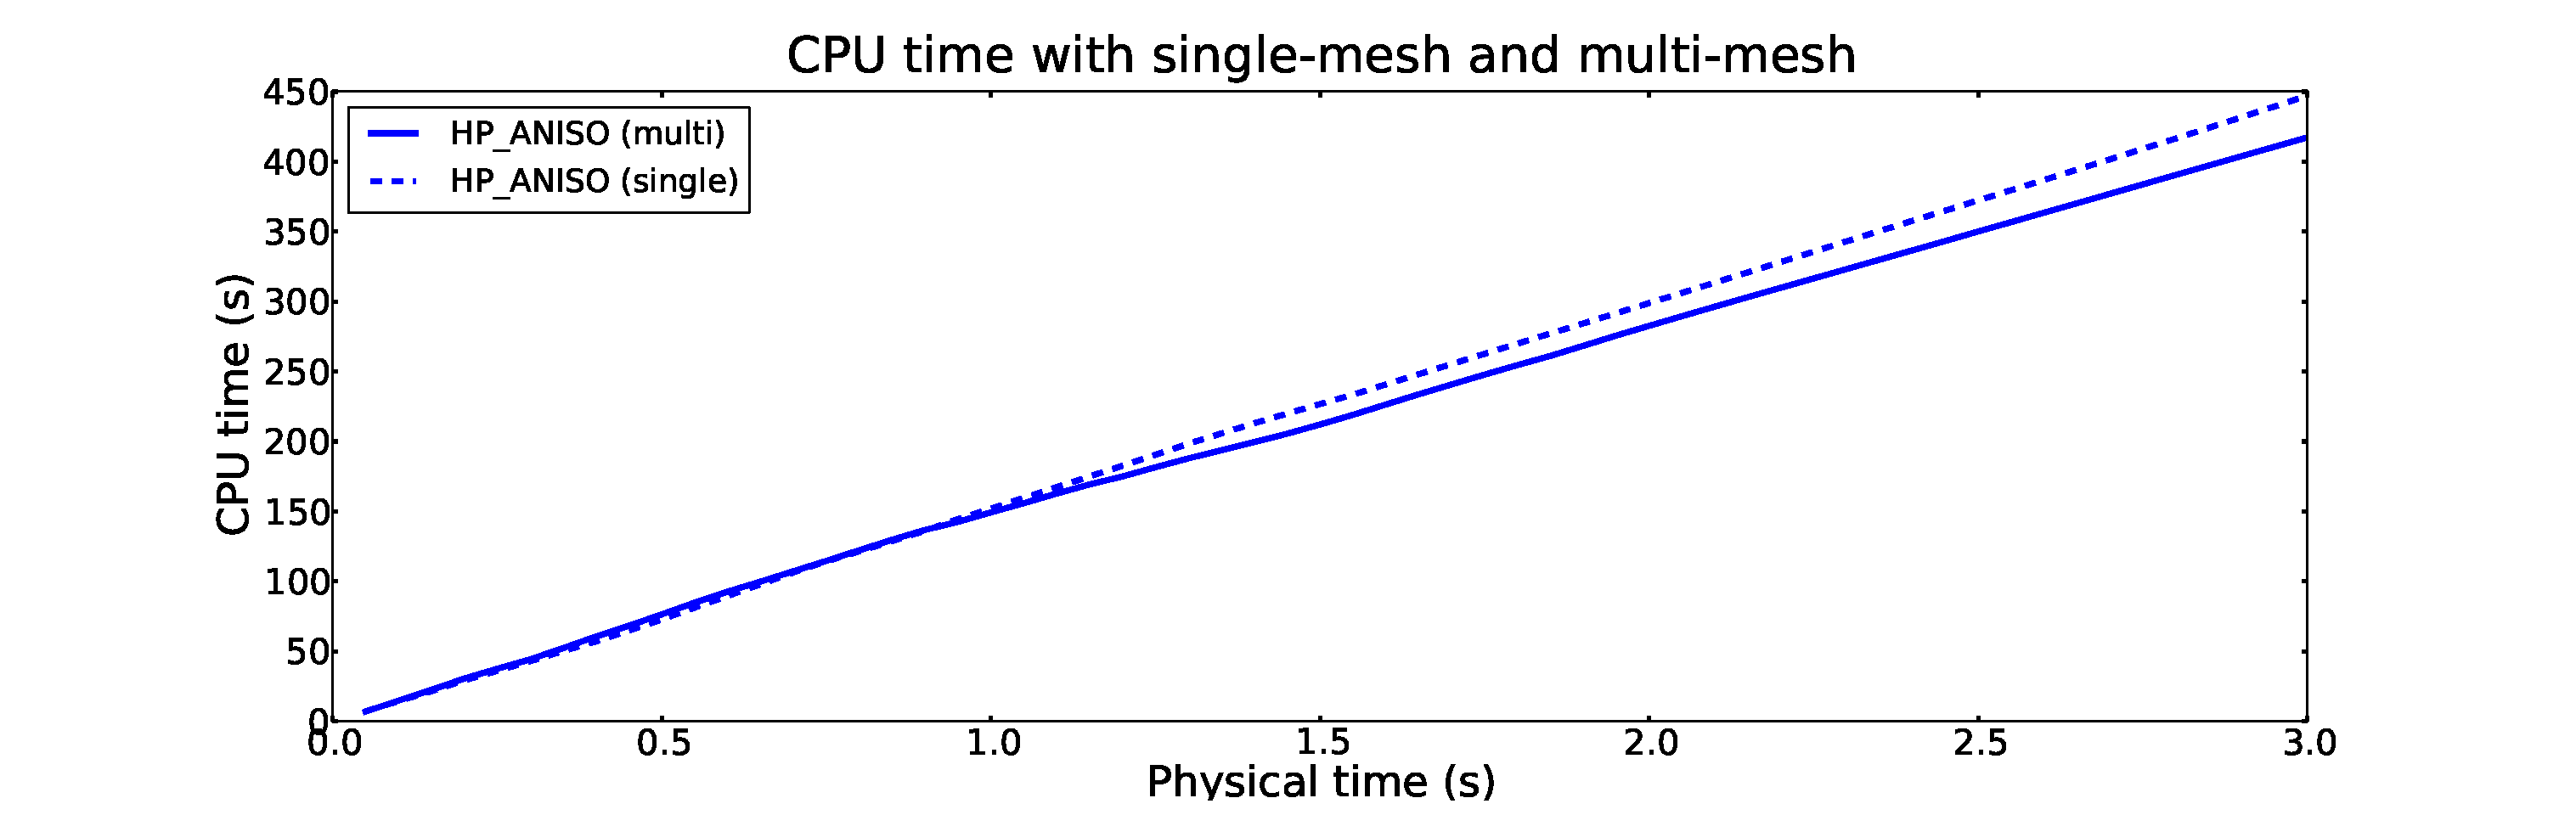
\includegraphics[width=\columnwidth]{singlemulti_cpu}
  \caption{\label{fig:singlemulticpu} Cumulative CPU time as a function 
  of physical time for single-mesh and multi-mesh configurations with 
  HP\_ANISO adaptivity mode.}
  \end{centering}
\end{figure}

\noindent 
Figs.~\ref{fig:poly} and~\ref{fig:poly2} show higher-order meshes in the adaptive multi-mesh $hp$-FEM
computation for $c$ and $\varphi$ at $t = 0.1$~s and $t=3.0$~s, respectively. Different 
colors mean different polynomial degrees. A diagonal pattern inside an element 
tells that the element has different polynomial degrees in the 
horizontal and vertical directions. 


\begin{figure}[!ht]
  \begin{centering}
  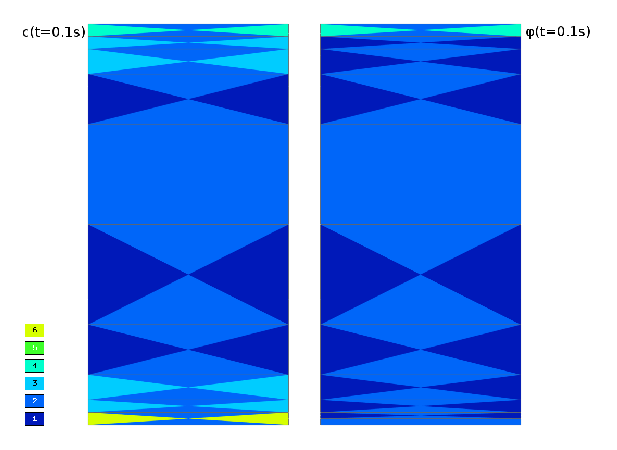
\includegraphics[width=.75\columnwidth]{poly}
  \caption{\label{fig:poly} Higher-order FEM mesh for 
  $c$ and $\varphi$ at $t=0.1\ s$. }
  \end{centering}
\end{figure}

\begin{figure}[!ht]
  \begin{centering}
  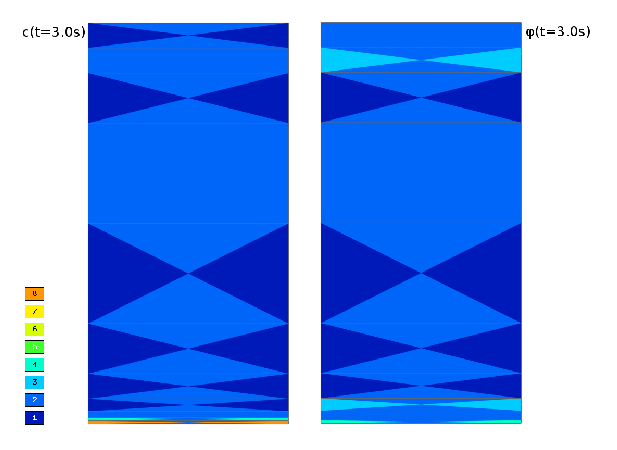
\includegraphics[width=.75\columnwidth]{poly2}
  \caption{\label{fig:poly2} Higher-order FEM mesh for 
  $c$ and $\varphi$ at $t=3.0\ s$. }
  \end{centering}
\end{figure}
\noindent
The result are in good agreement with Fig.~\ref{fig:cphi-2} --- in the vicinity
of the boundaries $\partial \Omega_1$ and $\partial\Omega_3$, the concentration gradient
is much greater than the voltage gradient. Therefore at $t=0.1$~s, 
the multi-mesh $hp$-FEM adaptivity 
algorithm has increased the maximum polynomial degree for the $c$-space to~6 while 
the maximum polynomial degree for the $\varphi$-space is~4. The meshes are not
that different in the beginning of the calculation. However, one can also see that the mesh 
refinement for $c$ at $t=3.0$~s is notably different compared to $\varphi$. For instance,
the highest polynomial degree for $c$-space is~8 whereas for $\varphi$-space is~4.
Since these results are representative for all adaptivity modes, only multi-mesh 
configurations are considered in the following. 

\subsection{Comparison of isotropic and anisotropic refinements}

Next we would like to illustrate the role of anisotropic mesh refinements.
Figs.~\ref{fig:isoanisodof} and \ref{fig:isoanisocpu} show typical results 
for the HP\_ISO, HP\_ANISO\_H,  HP\_ANISO adaptivity modes in terms 
of DOF and cumulative CPU time. Fig.~\ref{fig:isoanisoerror} shows corresponding
error convergence. It can be seen that HP\_ISO is notoriously inefficient as the
error does not converge within the limited number of degrees of freedom 
of $nDOF_{threshold}=5000$ and computing time is very large. Due to that fact,
the calculation of HP\_ISO was canceled before $t=3.0$~s.

\begin{figure}[!ht]
  \begin{centering}
  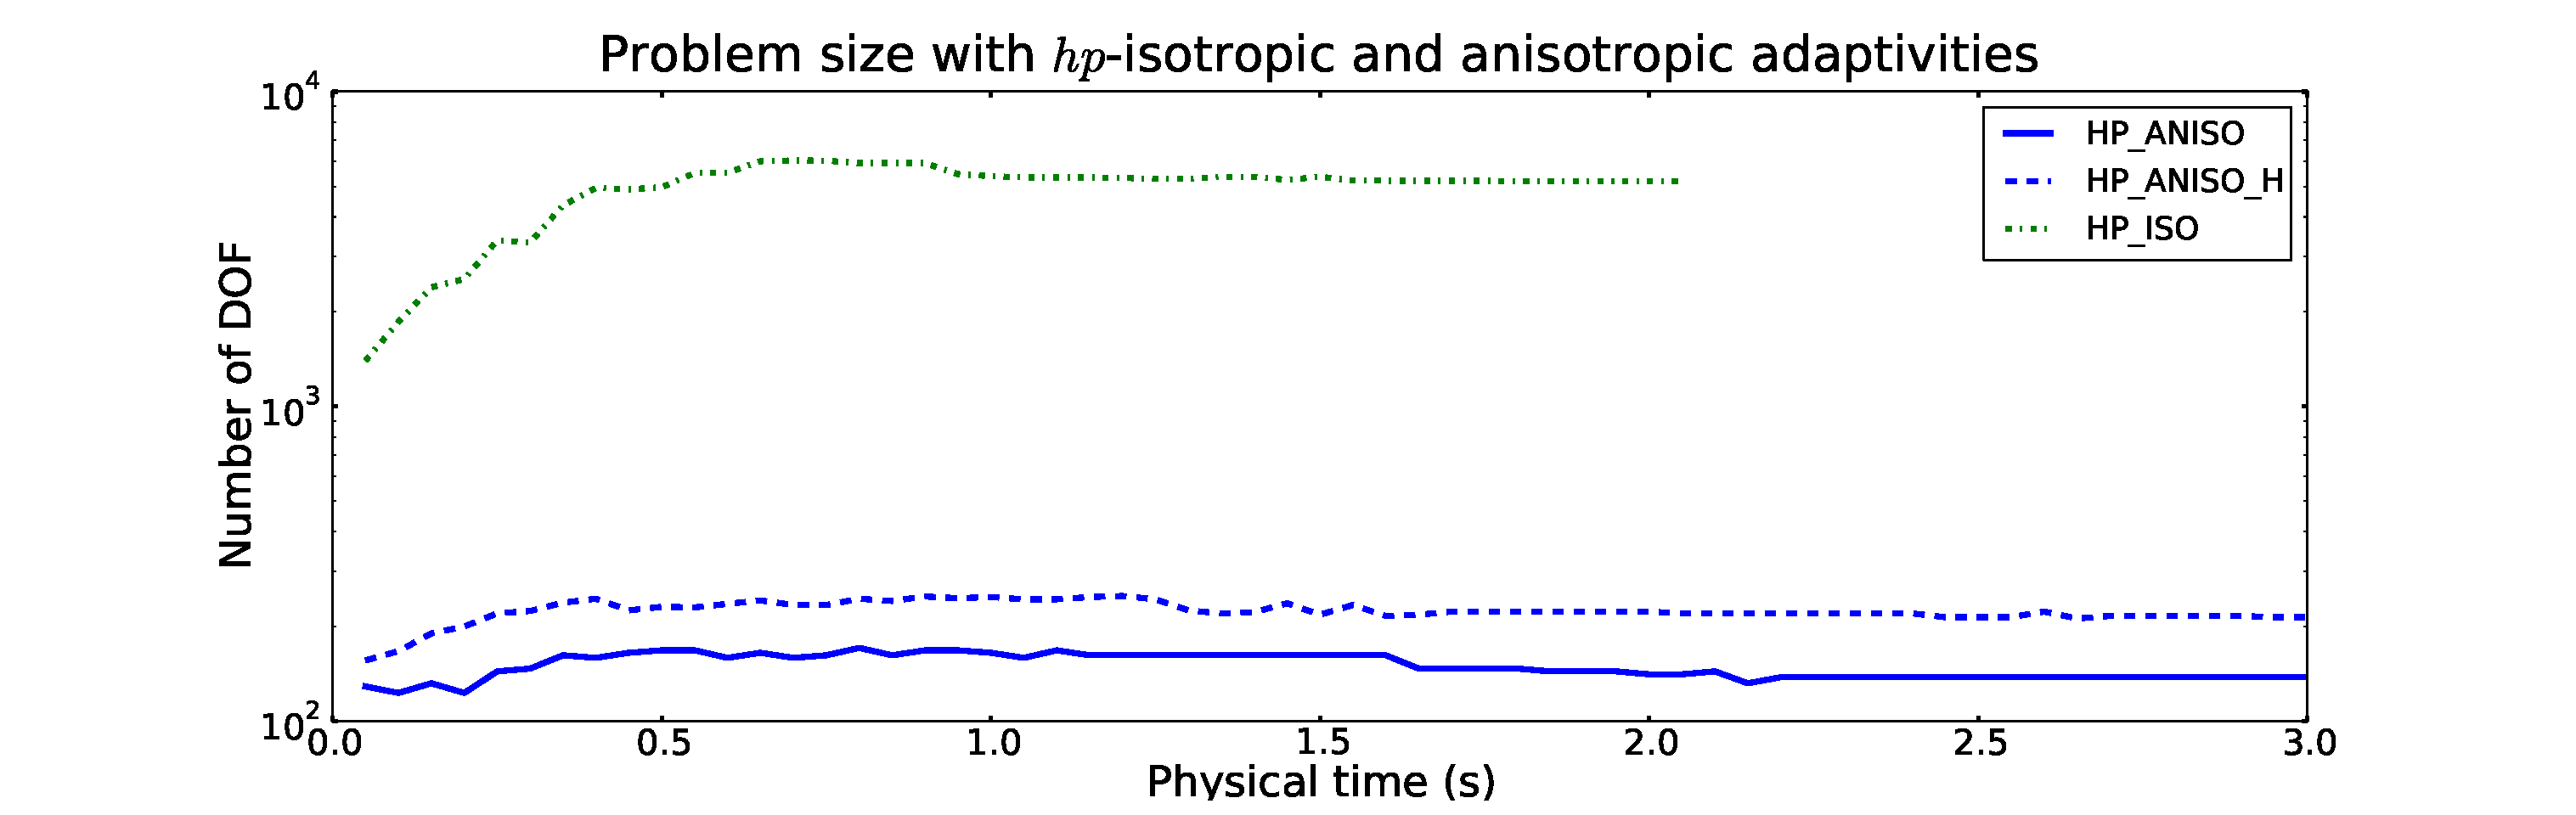
\includegraphics[width=\columnwidth]{isoaniso_dof}
  \caption{\label{fig:isoanisodof} Number of DOF as a function of physical time for 
  multi-mesh configurations with HP\_ANISO,
  HP\_ANISO\_H, and HP\_ISO adaptivity modes (log~$y$ scale).}
  \end{centering}
\end{figure}

\begin{figure}[!ht]
  \begin{centering}
  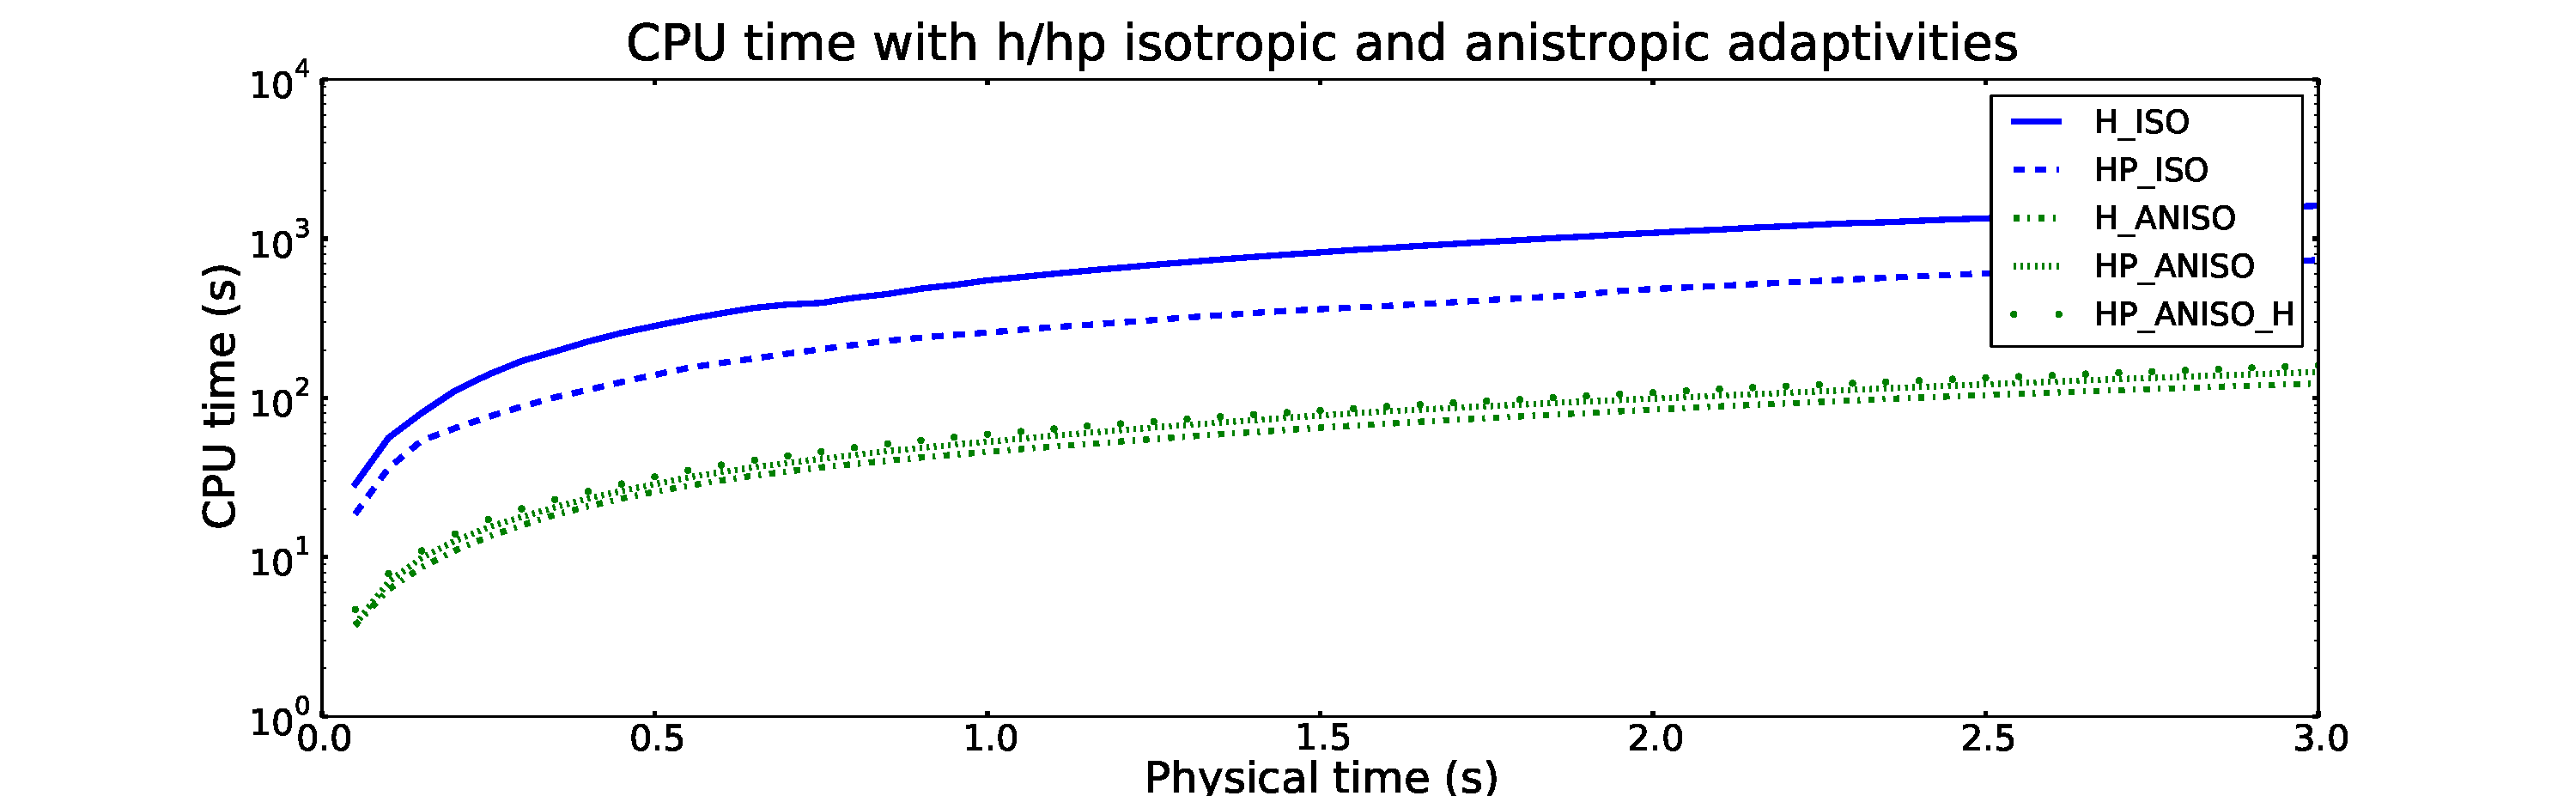
\includegraphics[width=\columnwidth]{isoaniso_cpu}
  \caption{\label{fig:isoanisocpu} Cumulative CPU time as a function of physical time 
  for multi-mesh configurations with HP\_ANISO,
  HP\_ANISO\_H, and HP\_ISO adaptivity modes (log~$y$ scale).}
  \end{centering}
\end{figure}

\begin{figure}[!ht]
  \begin{centering}
  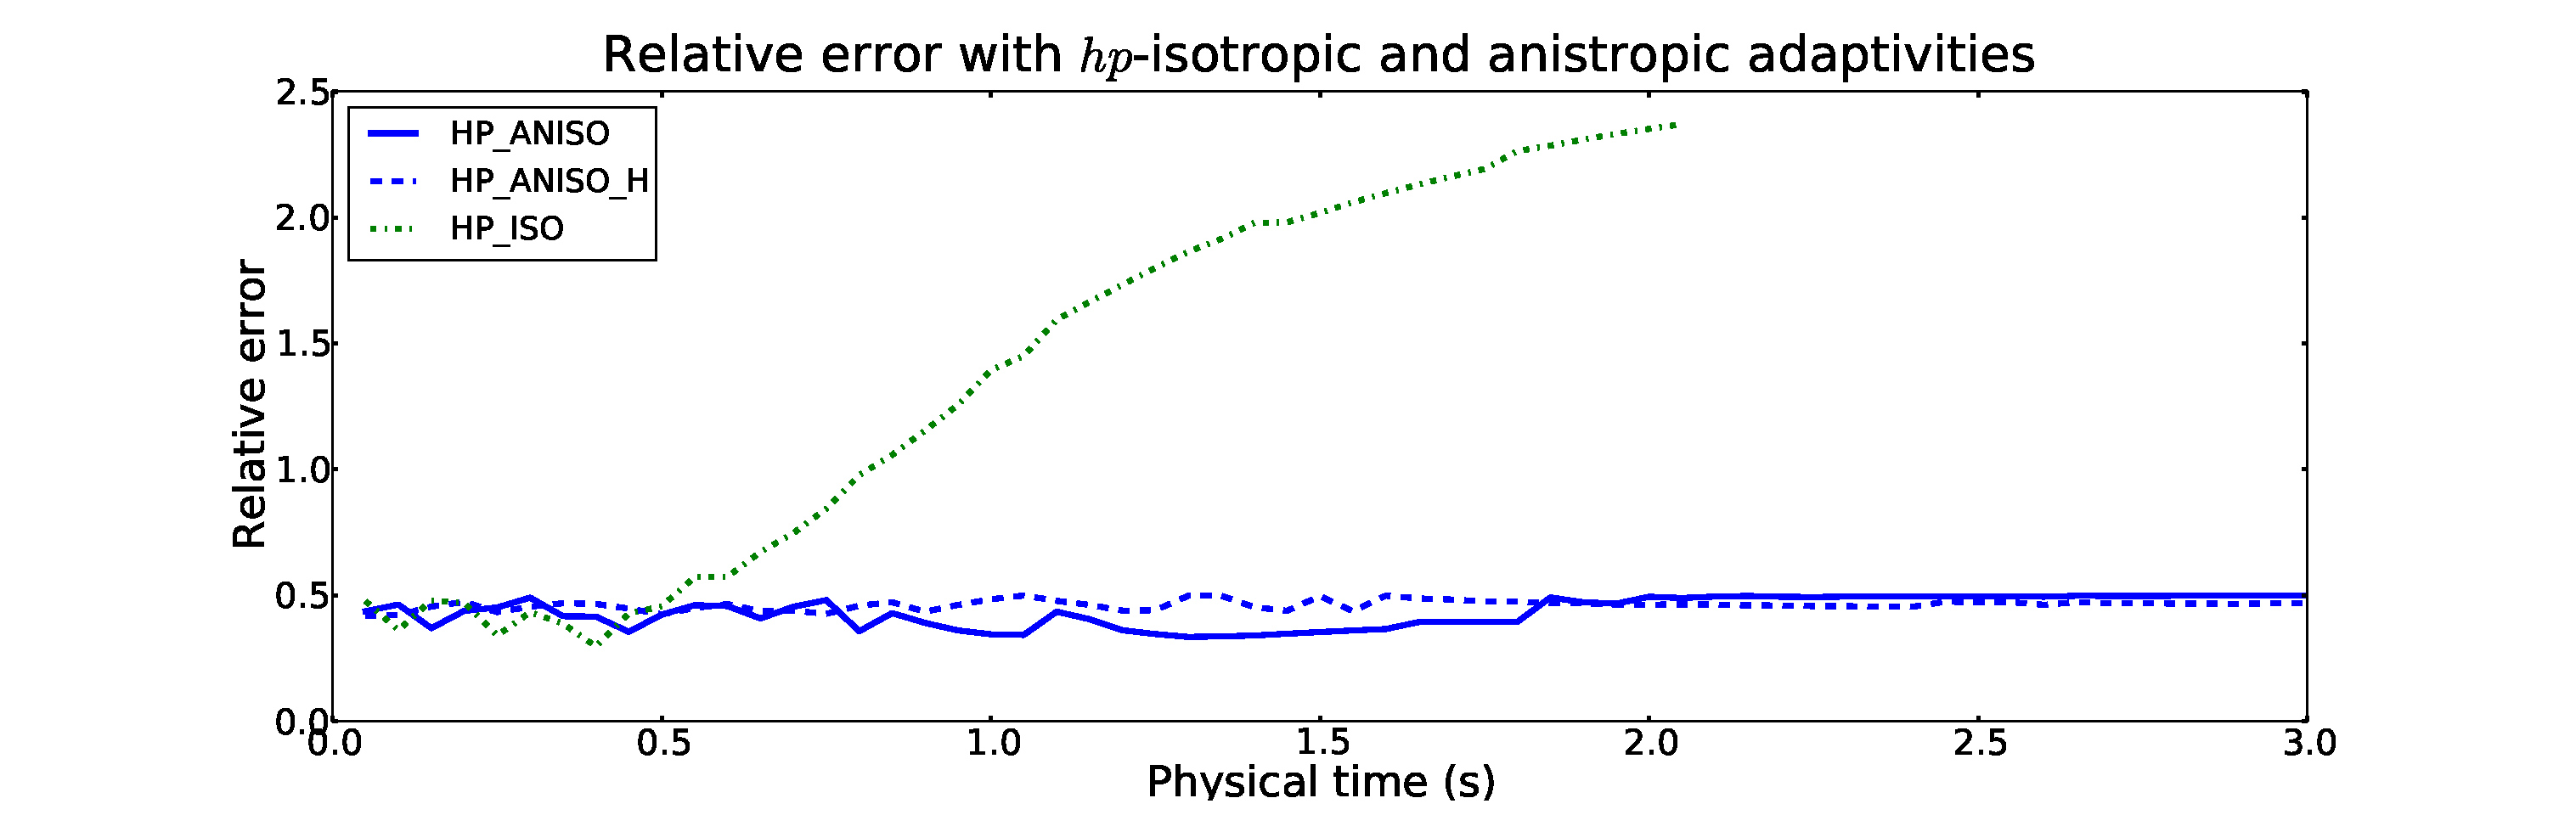
\includegraphics[width=\columnwidth]{isoaniso_error}
  \caption{\label{fig:isoanisoerror} Relative solution error as a function of physical time 
  for multi-mesh configurations with HP\_ANISO,
  HP\_ANISO\_H, and HP\_ISO adaptivity modes.}
  \end{centering}
\end{figure}

\noindent
Figs.~\ref{fig:isoanisopdof} and \ref{fig:isoanisopcpu} present a similar 
comparison for the P\_ISO, P\_ANISO, and HP\_ANISO\_P modes. Recall that these 
computations use a different initial mesh that was a-priori refined in space.

%\newpage

\begin{figure}[!ht]
  \begin{centering}
  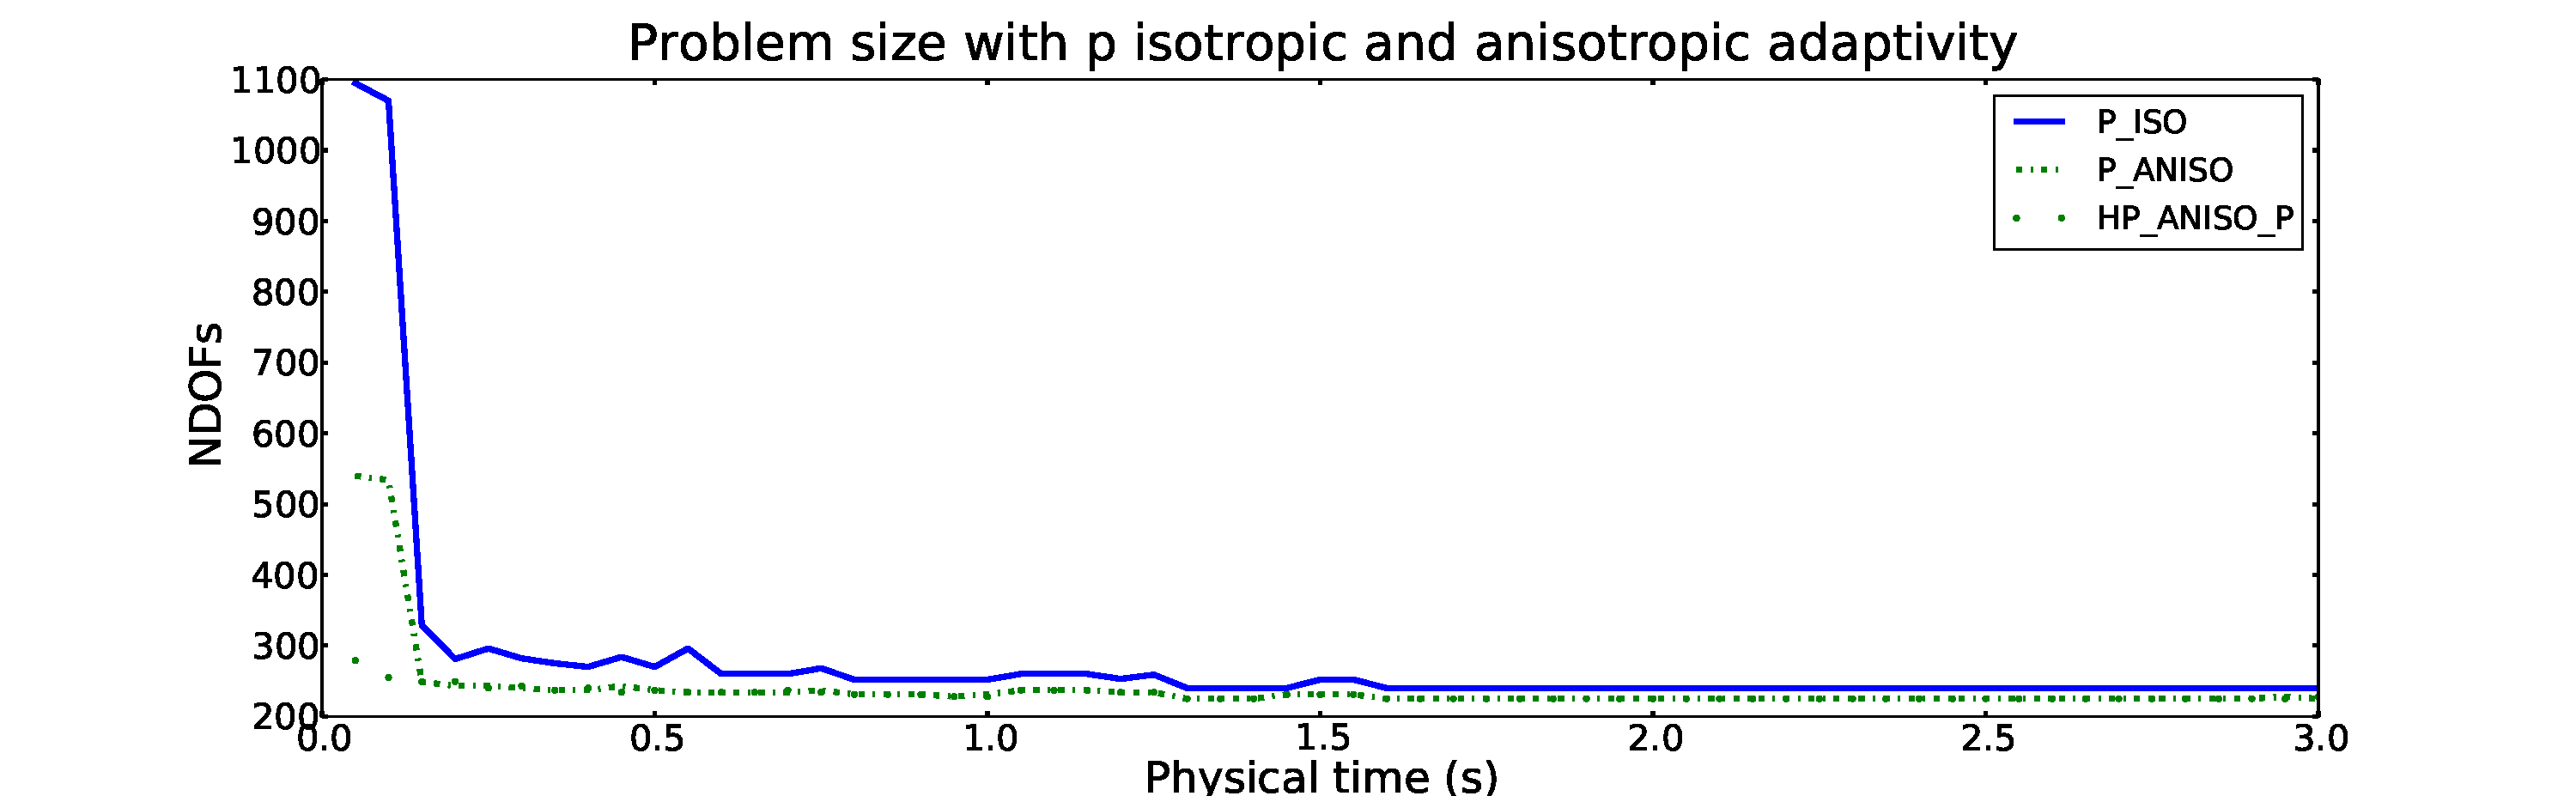
\includegraphics[width=\columnwidth]{isoanisop_dof}
  \caption{\label{fig:isoanisopdof} Number of DOF as a function of physical time
  for multi-mesh configurations with P\_ISO, P\_ANISO, and
  HP\_ANISO\_P adaptivity modes.}
  \end{centering}
\end{figure}

\begin{figure}[!ht]
  \begin{centering}
  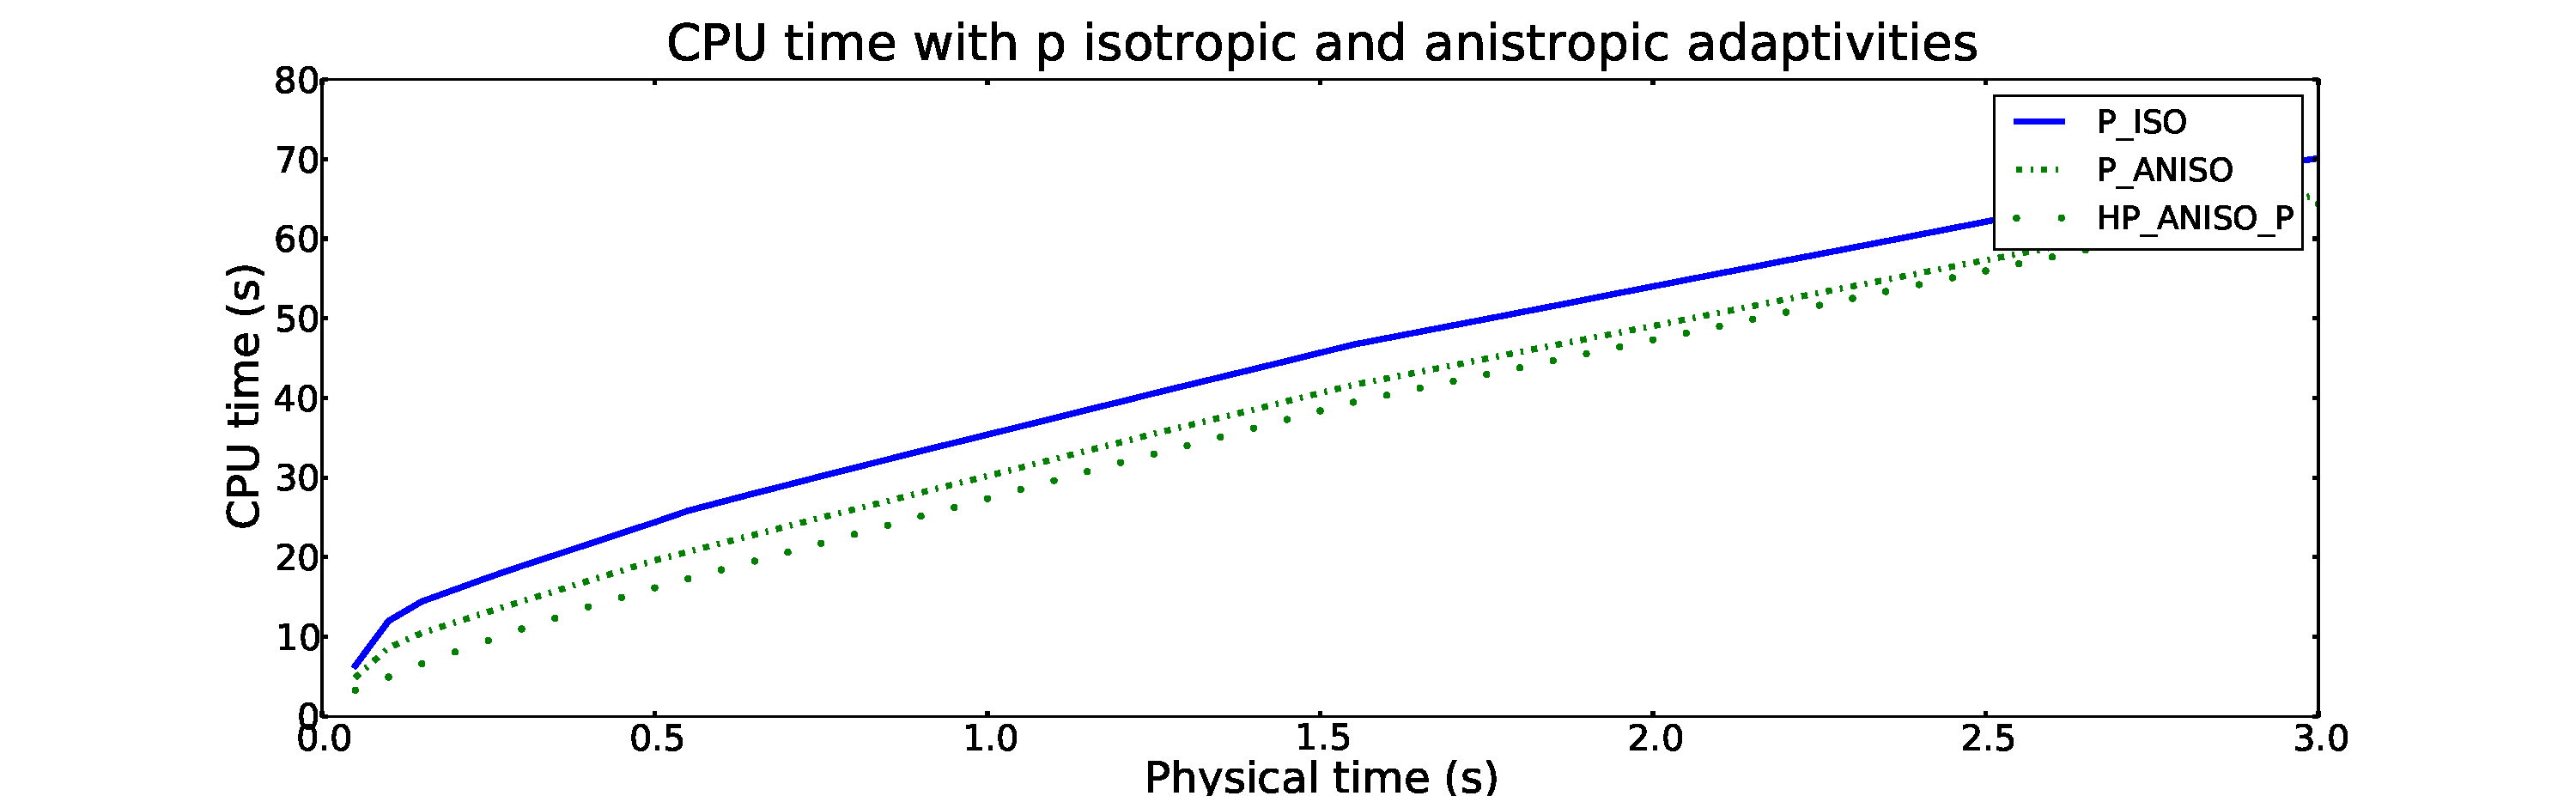
\includegraphics[width=\columnwidth]{isoanisop_cpu}
  \caption{\label{fig:isoanisopcpu} Cumulative CPU times as a function of physical time
  for multi-mesh configurations with P\_ISO, P\_ANISO, and
  HP\_ANISO\_P adaptivity modes.}
  \end{centering}
\end{figure}

As a conclusion, the reader can see that the anisotropic adaptivity modes always perform better than 
the isotropic ones. In particular, HP\_ANISO results into the smallest problem size. 
In the \emph{p}-adaptivity group, HP\_ANISO\_P and P\_ANISO lead to a small problem size
consistently in each time step, whereas P\_ISO yields large problems
during the first time steps. 

HP\_ANISO also results in the fastest
computing time among $hp$-adaptivity group whereas HP\_ANISO\_P
results in the fastest overall computing time. This is due to the fact
that HP\_ANISO\_P calculation is performed on the refined mesh. 
Regardless, the HP\_ANISO adaptivity mode is the most suitable
for the PNP problem due to the small size and relative fastness compared
to the other adaptivity modes. A way to optimize the computing time
of HP\_ANISO will be considered next.

\subsection{Time step control of HP\_ANISO adaptivity}

\begin{figure}[!ht]
  \begin{centering}
  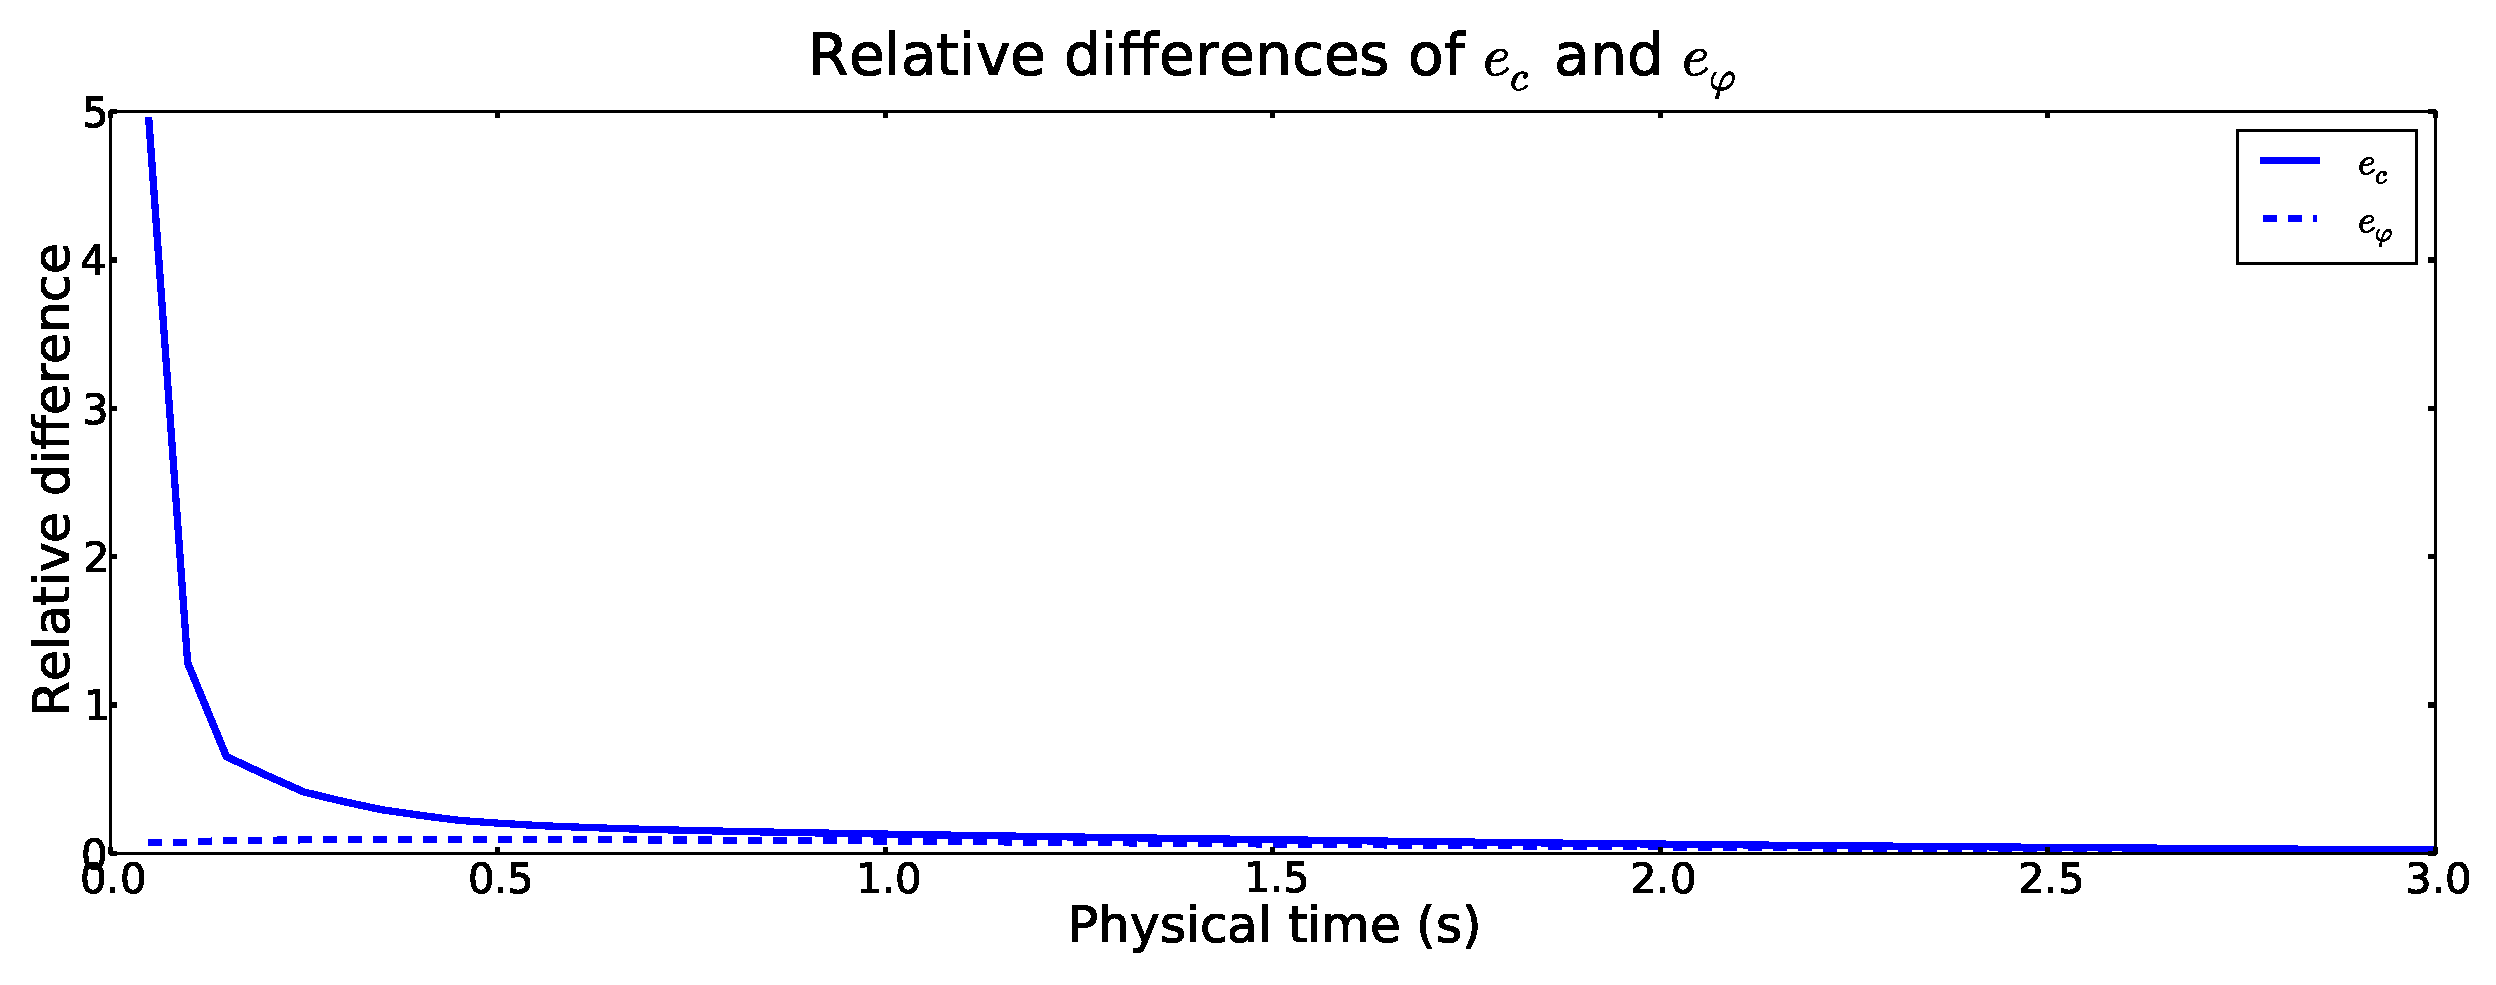
\includegraphics[width=\columnwidth]{cphi_relerr}
  \caption{\label{fig:cphirelerr} Relative difference $e_{c}^n$ and $e_{\varphi}^n$.}
  \end{centering}
\end{figure}
\begin{figure}[!ht]
  \begin{centering}
  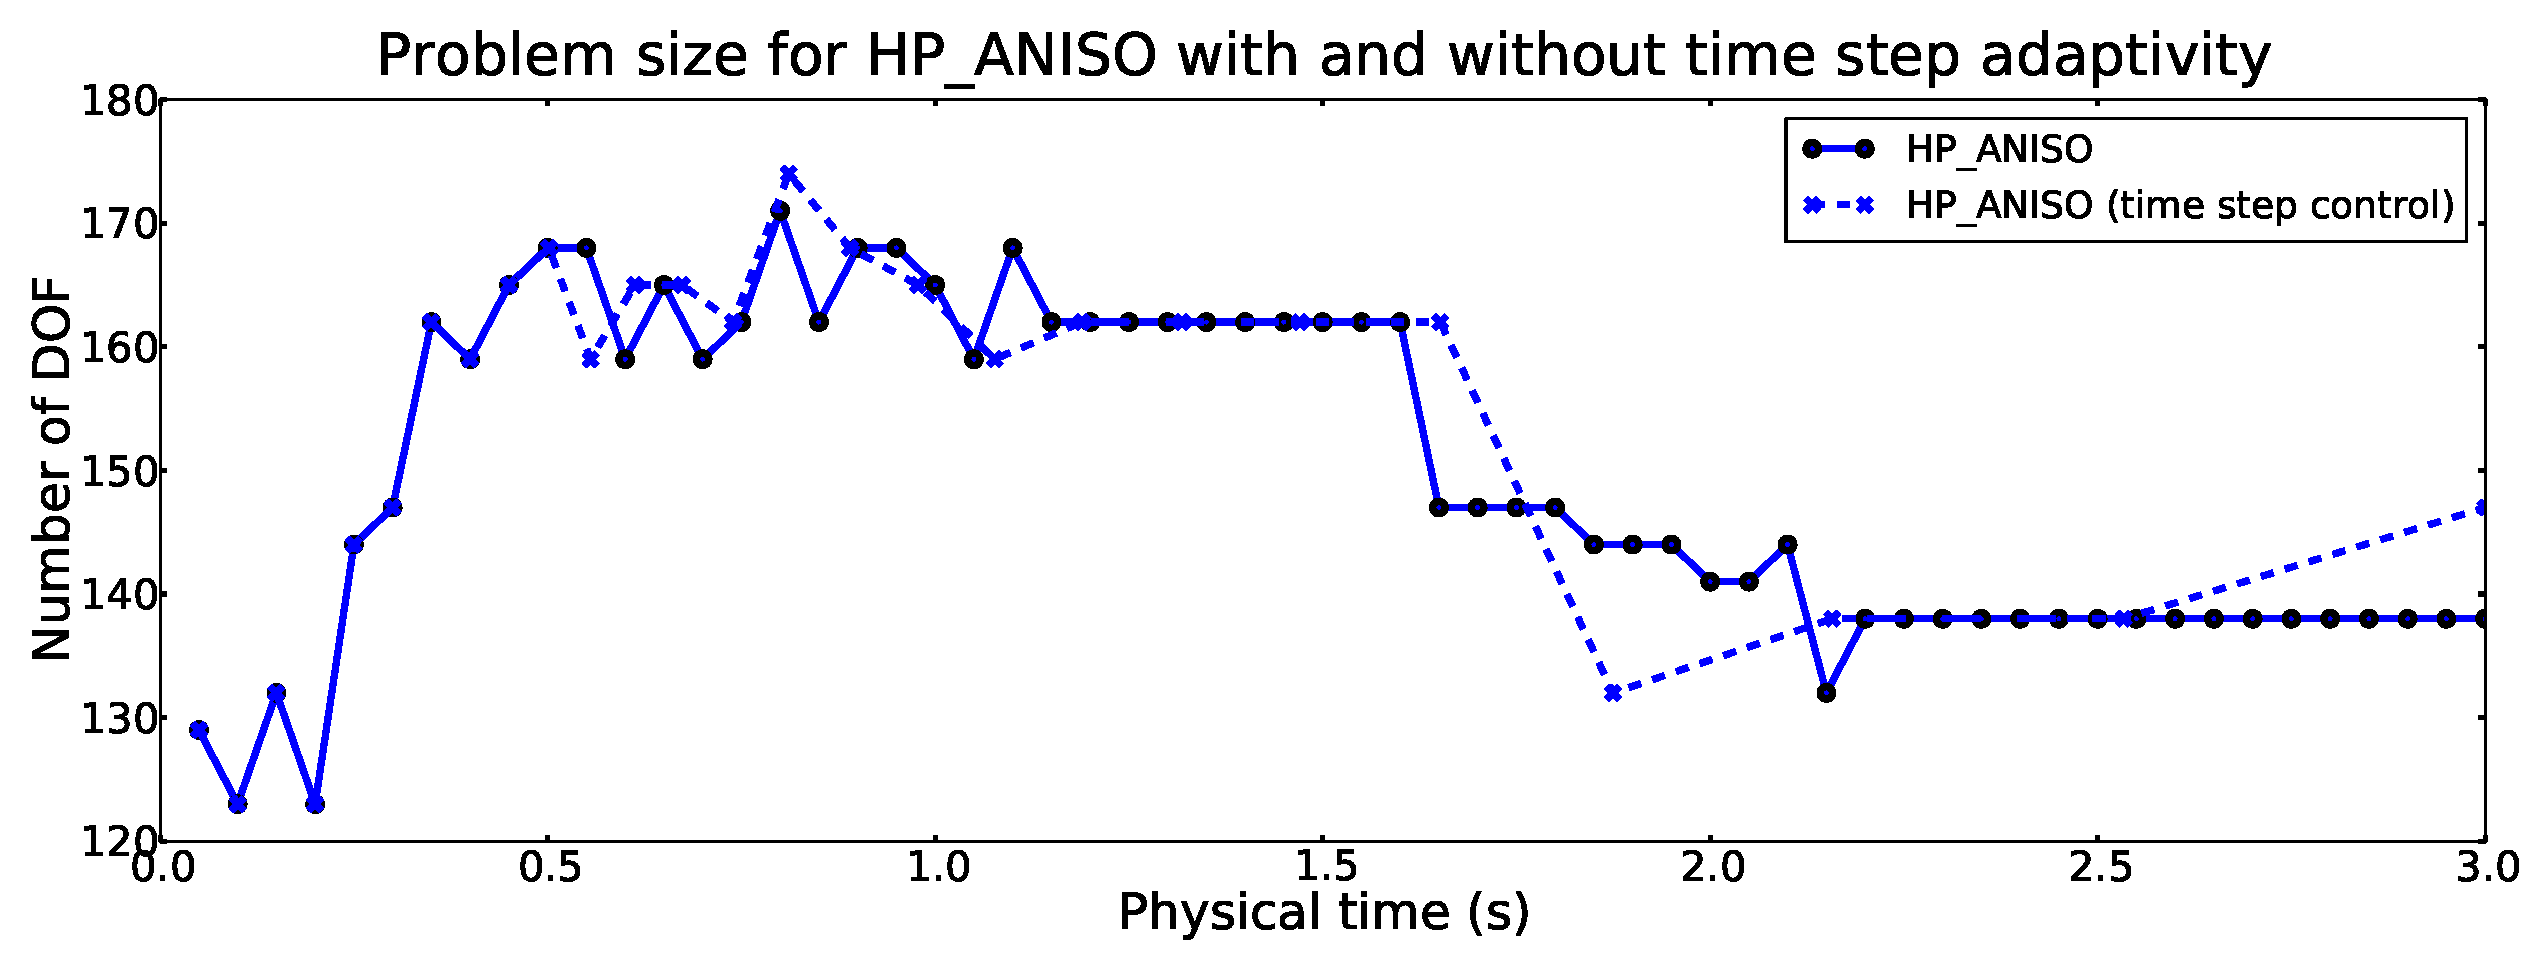
\includegraphics[width=\columnwidth]{timeadapt_dof}
  \caption{\label{fig:timeadapt_dof} Number of DOF
  as a function of physical time for HP\_ANISO with and without
  time step adaptivity. The markers on the graphs indicate the
  time steps.}
  \end{centering}
\end{figure}
\begin{figure}[!ht]
  \begin{centering}
  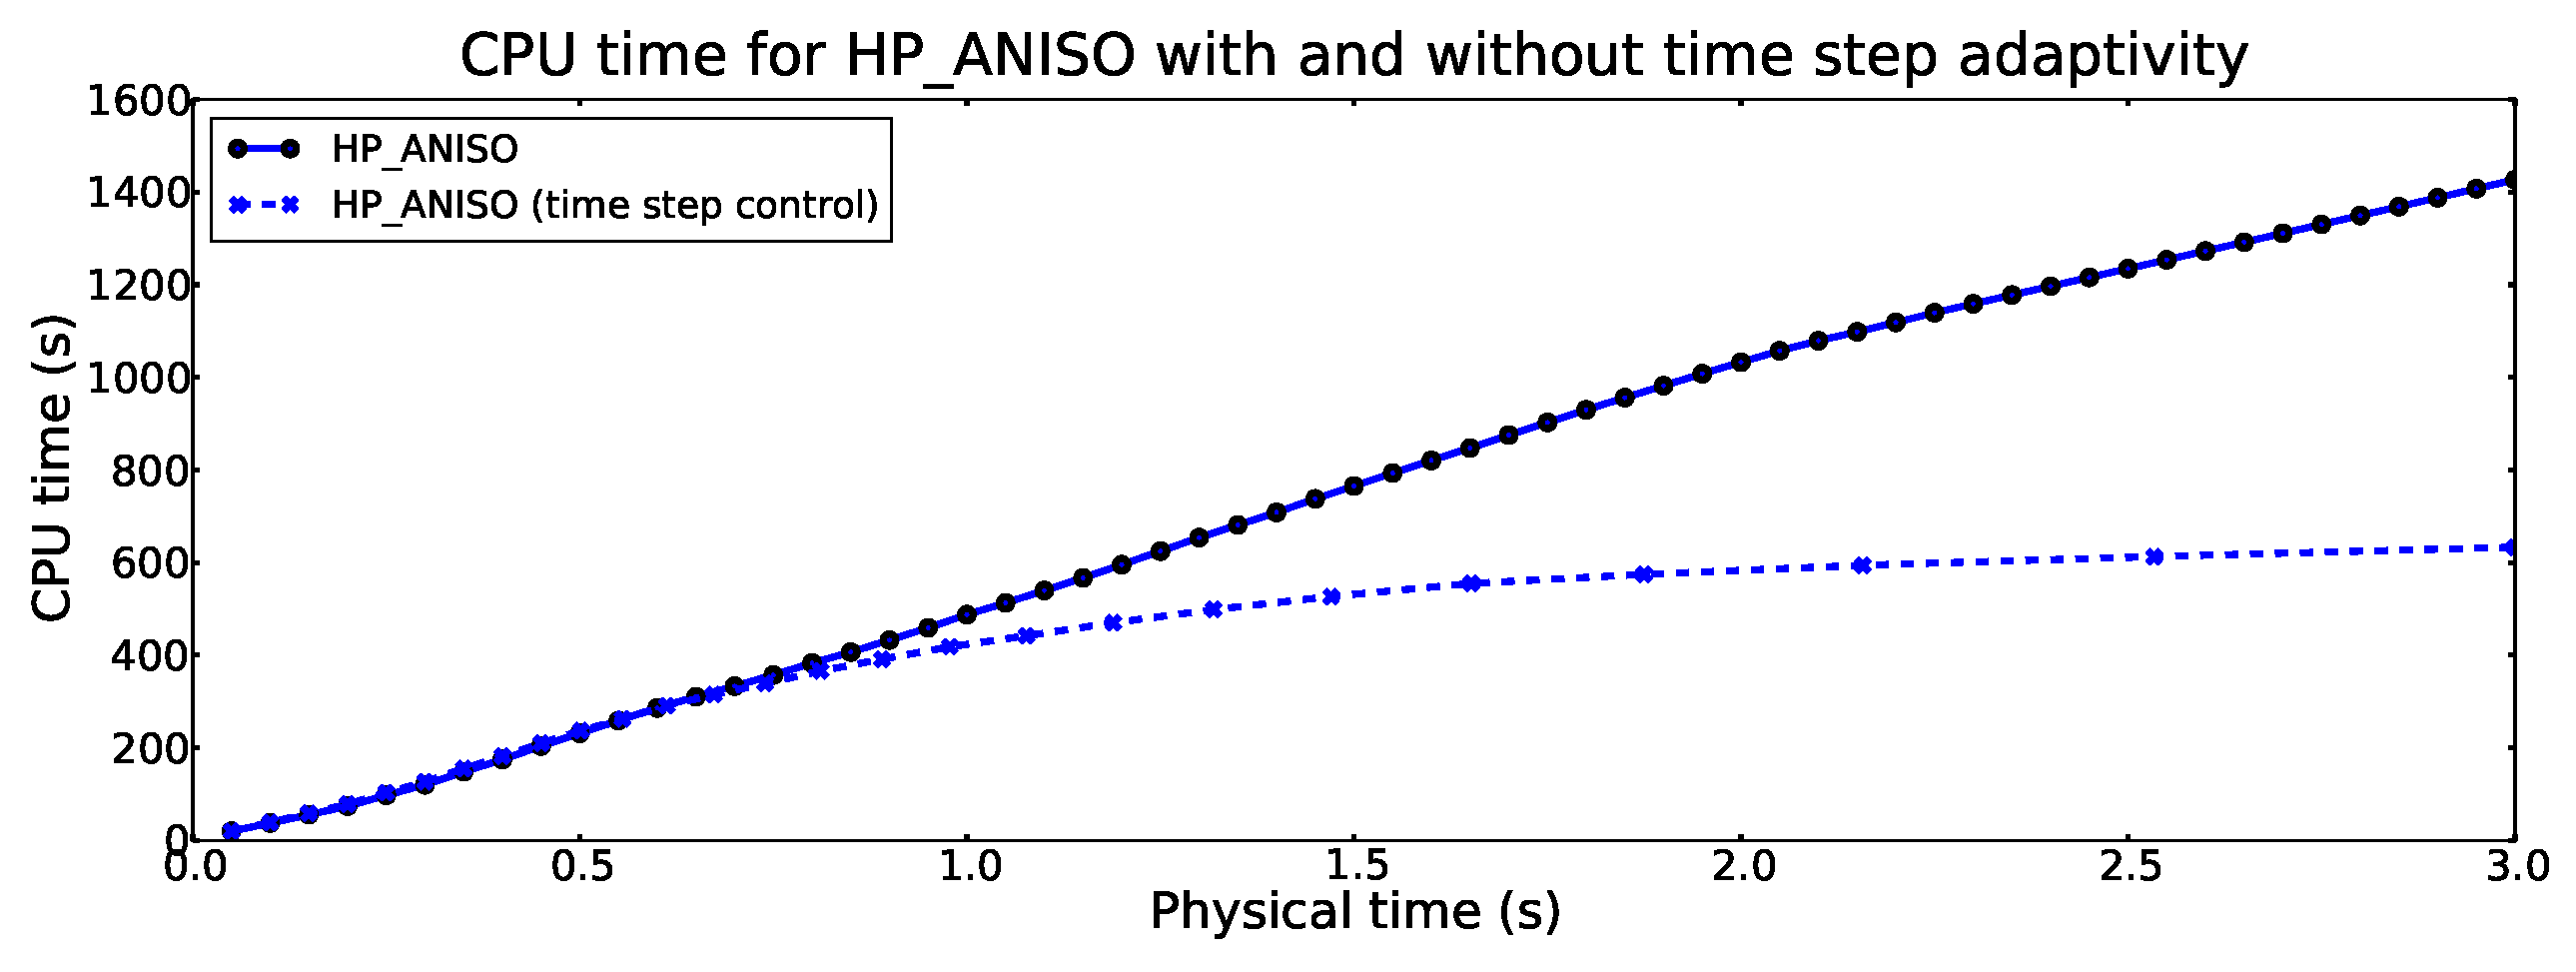
\includegraphics[width=\columnwidth]{timeadapt_cpu}
  \caption{\label{fig:timeadapt_cpu} Cumulative CPU times
  as a function of physical time for HP\_ANISO with and without
  time step adaptivity. The markers on the graphs indicate the
  time steps.}
  \end{centering}
\end{figure}

To optimize the calculation time of HP\_ANISO, an adaptive time step control was employed.
The classical PID controller was used~\cite{valli2002control,dubcova2010space}.
Since $c$ and $\varphi$ change differently in time as was demonstrated in Figs.~\ref{fig:cphi-1}
and~\ref{fig:cphi-2}, the relative changes between the solutions at different
time steps were monitored:
\begin{eqnarray}
  e_c^n & = & \frac{\lVert c^n-c^{n-1}\rVert}{\lVert c^n \rVert},\\
  e_\varphi^n & = & \frac{\lVert \varphi^n-\varphi^{n-1}\rVert}{\lVert \varphi^n \rVert}.
\end{eqnarray}
The relative changes to control the time step was calculated as follows:
\begin{equation}
  e^n=\max\left\{ e_c^n,\ e_\varphi^n \right\}.
\end{equation}
If $e^n < \delta$ where $\delta>0$ is a defined tolerance, then the time
step for the next iteration is increased smoothly to
\begin{equation}
  \delta\tau^{n+1}=\left( \frac{e^{n-1}}{e^n} \right)^{k_P}\ \left( \frac{\delta}{e^n} \right)^{k_l}\
  \left[ \frac{\left( e^{n-1} \right)^2}{e^n e^{n-2}} \right]^{k_D} \delta\tau^n,
\end{equation}
where parameters are from~\cite{valli2002control}:
\begin{equation}
  k_p=0.075,\quad k_l=0.175,\quad k_D=0.01.
\end{equation}
The tolerance $\delta$ was set to $\delta=0.25$ in the current optimization
example. At this point, the implementation does not support
adaptive time stepping if $e^n\geq \delta$. However, the implementation 
of advanced adaptive higher-order time-stepping methods is in progress.
The calculated $e_c^n$ and $e_\varphi^n$ are shown in Fig.~\ref{fig:cphirelerr}.
The HP\_ANISO problem size and computing time with and without time step control
are shown in Figs.~\ref{fig:timeadapt_dof} and~\ref{fig:timeadapt_cpu}. The reader
can notice that the computing time was reduced more than two times when the time
step control was employed.

\subsection{HP\_ANISO adaptivity with physically more realistic boundary conditions}
\begin{figure}[!ht]
  \begin{centering}
  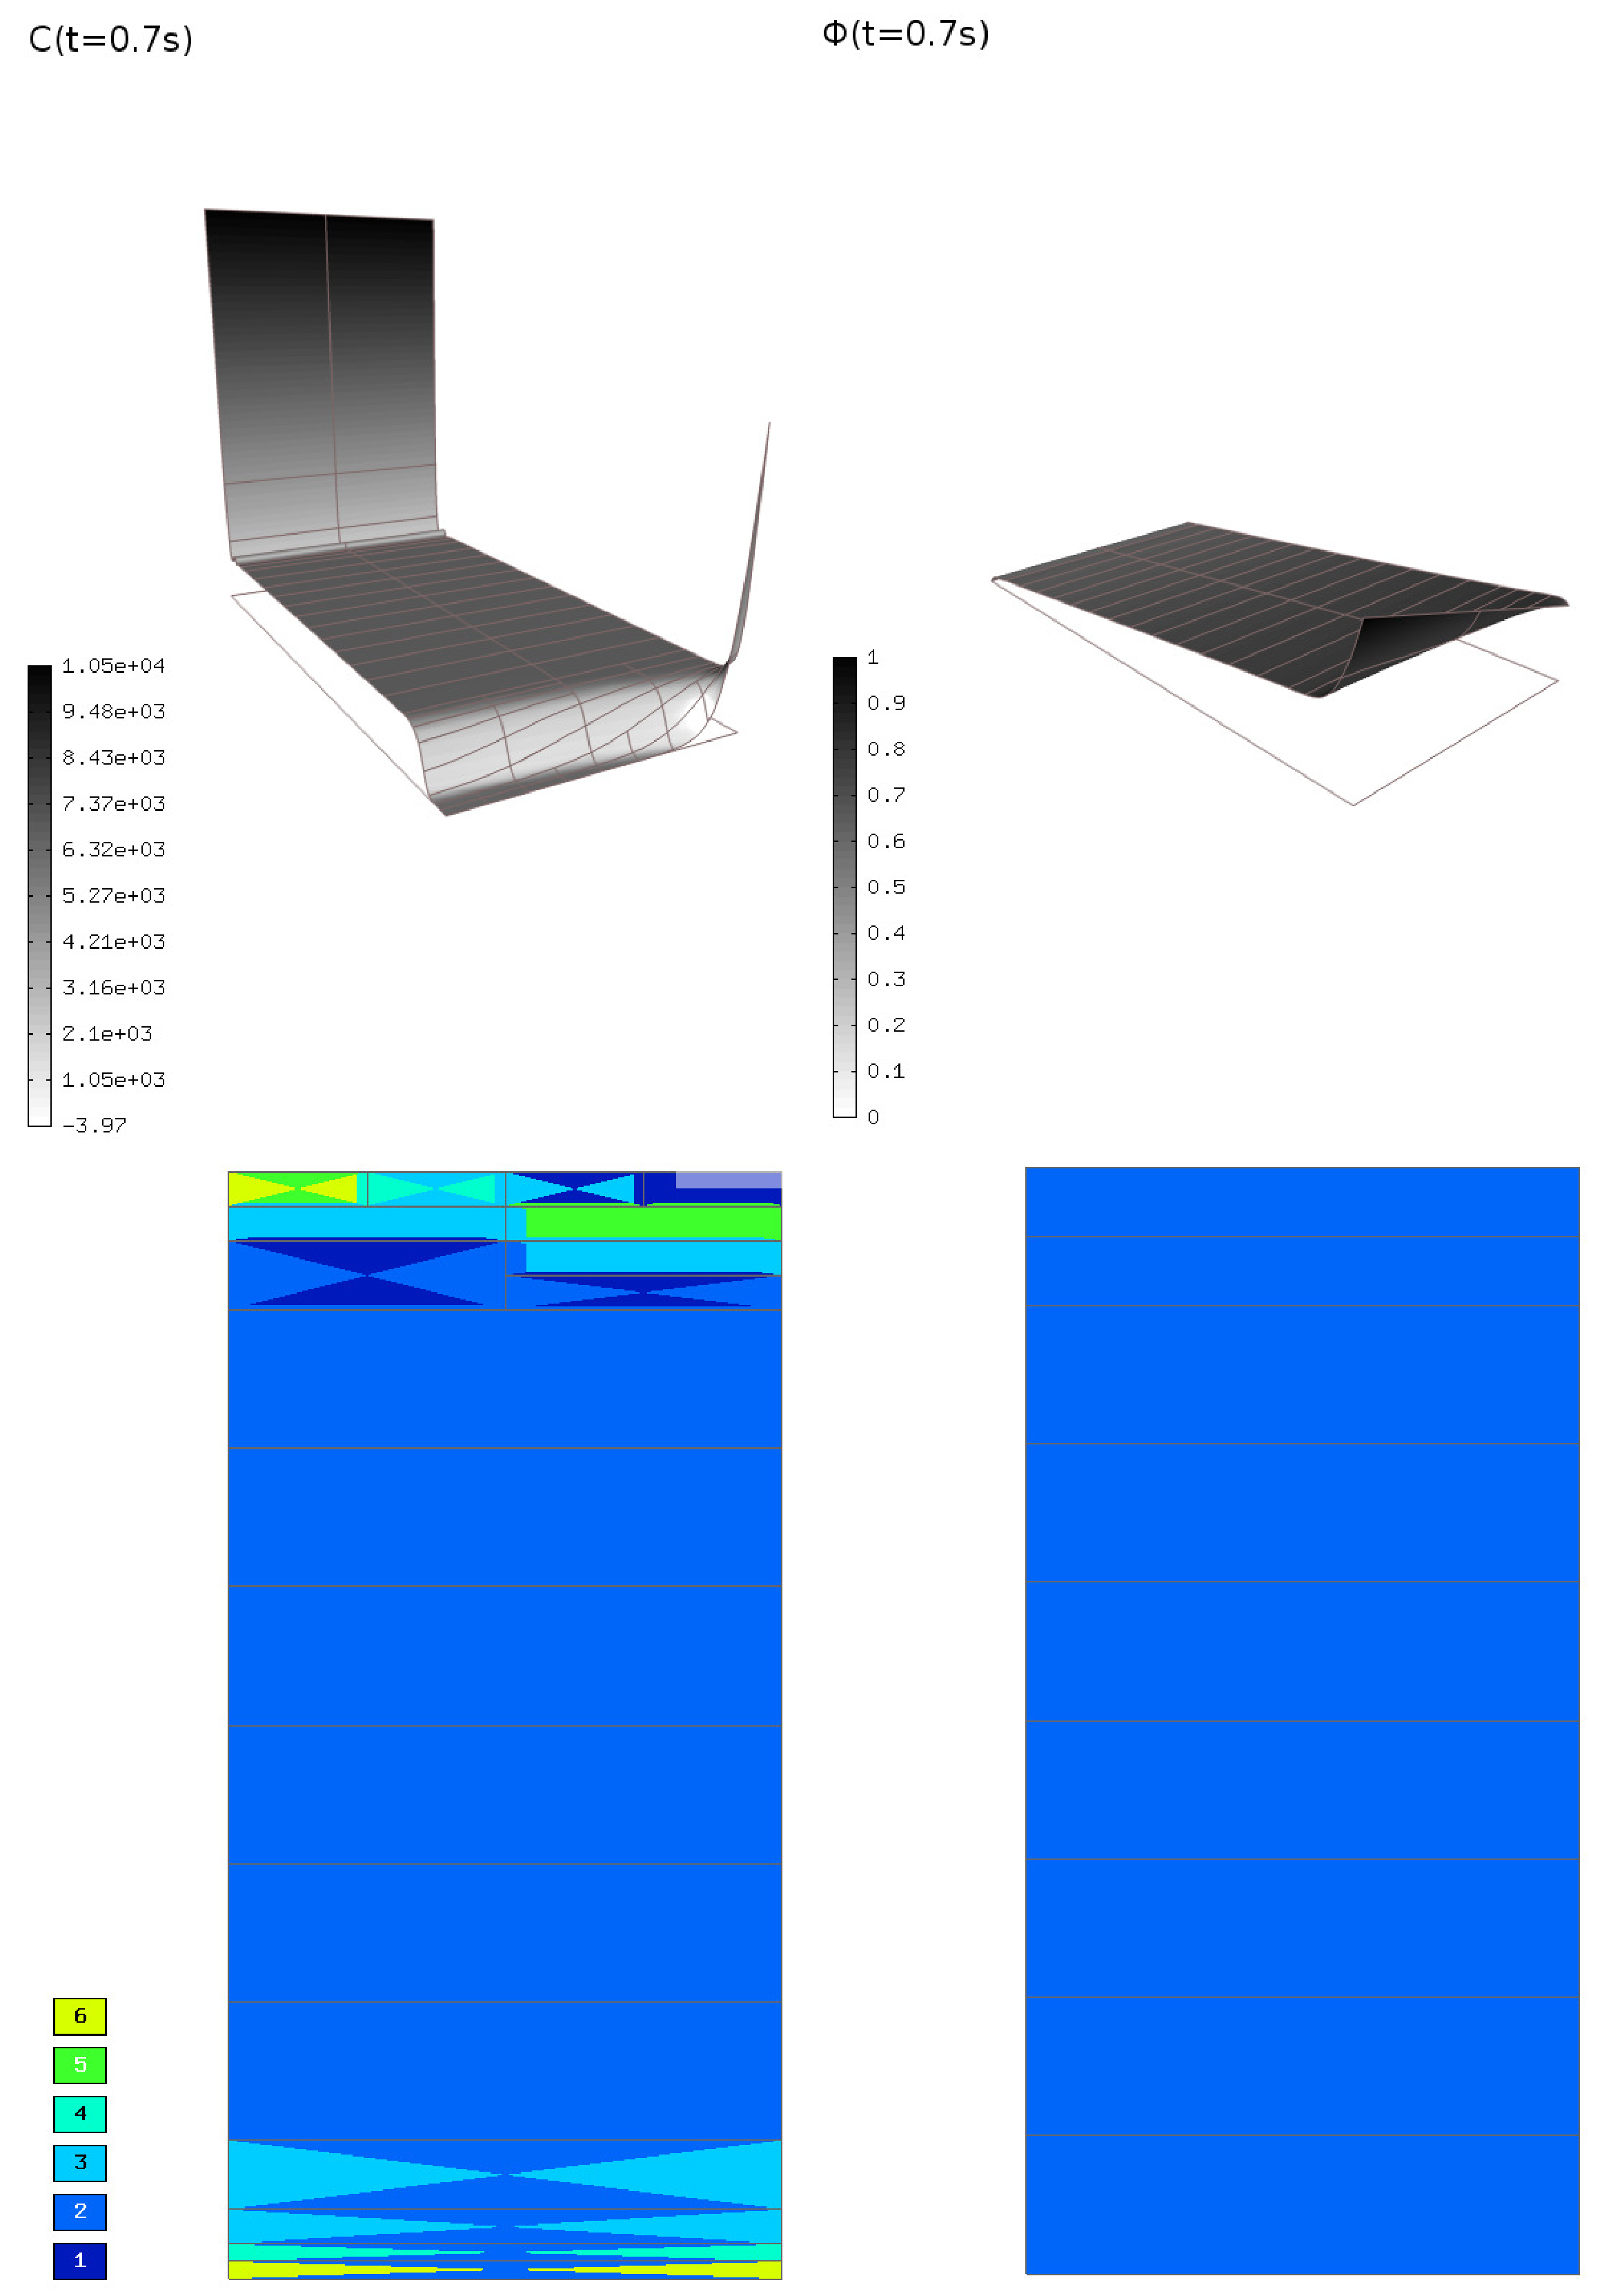
\includegraphics[width=\columnwidth]{cphiorders}
  \caption{\label{fig:cphi-orders} Solutions $c$ and $\varphi$
  and corresponding polynomial degrees of the elements at
  $t=0.1\ s$. HP\_ANISO refinement mode was used. The height
  in the solution graphs indicates the value.}
  \end{centering}
\end{figure}

In real physics calculations, the applied voltage on boundary $\partial\Omega_1$
is not constant. This can be, for instance, due to the high resistance of
the electrodes as explained in~\cite{pugal2009}.
To see how the HP\_ANISO adaptivity works for such situations, the
voltage on the boundary was applied as follows:
\begin{equation}
  \phi_{\Omega_1}\left( x \right)=0.5\left[V \right] \frac{x\left[ m \right ]}{\text{width}_{\Omega_1}\left[ m \right]}+0.5\left[ V \right],
\end{equation}
where $\text{width}_{\Omega_1}$ is the width of the boundary. The given boundary is effectively
a linear increase of the voltage from $\phi_{\Omega_1}\left(x = 0 \right)=0.5$~V to
$\phi_{\Omega_1}\left(x=\text{width}_{\Omega_1}\right) = 1.0$~V.
Now the concentration gradient $\nabla c$ and the voltage gradient $\nabla \varphi$ are no
longer effectively in 1D.

The calculated scaled values $c$ and $\varphi$ in $\Omega$ and corresponding meshes and polynomial
degrees of the elements at $t=0.1$~s are shown in Fig.~\ref{fig:cphi-orders}.
Notice that the solution
is different to the one in Fig.~\ref{fig:cphi-1}. The HP\_ANISO
adaptivity algorithm has particularly increased the polynomial degree
and refined the mesh near $\Omega_1$ where a sharp concentration
peak exists (compare to Fig.~\ref{fig:poly}).
At $t=3.0$~s, the shape of the solutions $c$ and $\varphi$ are similar to the one
in Fig.~\ref{fig:cphi-2} and therefore the polynomial space and mesh gets adapted
accordingly. This example clearly illustrates how 
the solution of PNP with non-uniform
boundary conditions is very dynamic in time
and how the HP\_ANISO time dependent adaptivity 
finds an optimal mesh and polynomial space to adapt to the dynamics
of the problem. 

\subsection{Length scale analysis}

\begin{figure}[!ht]
  \begin{centering}
  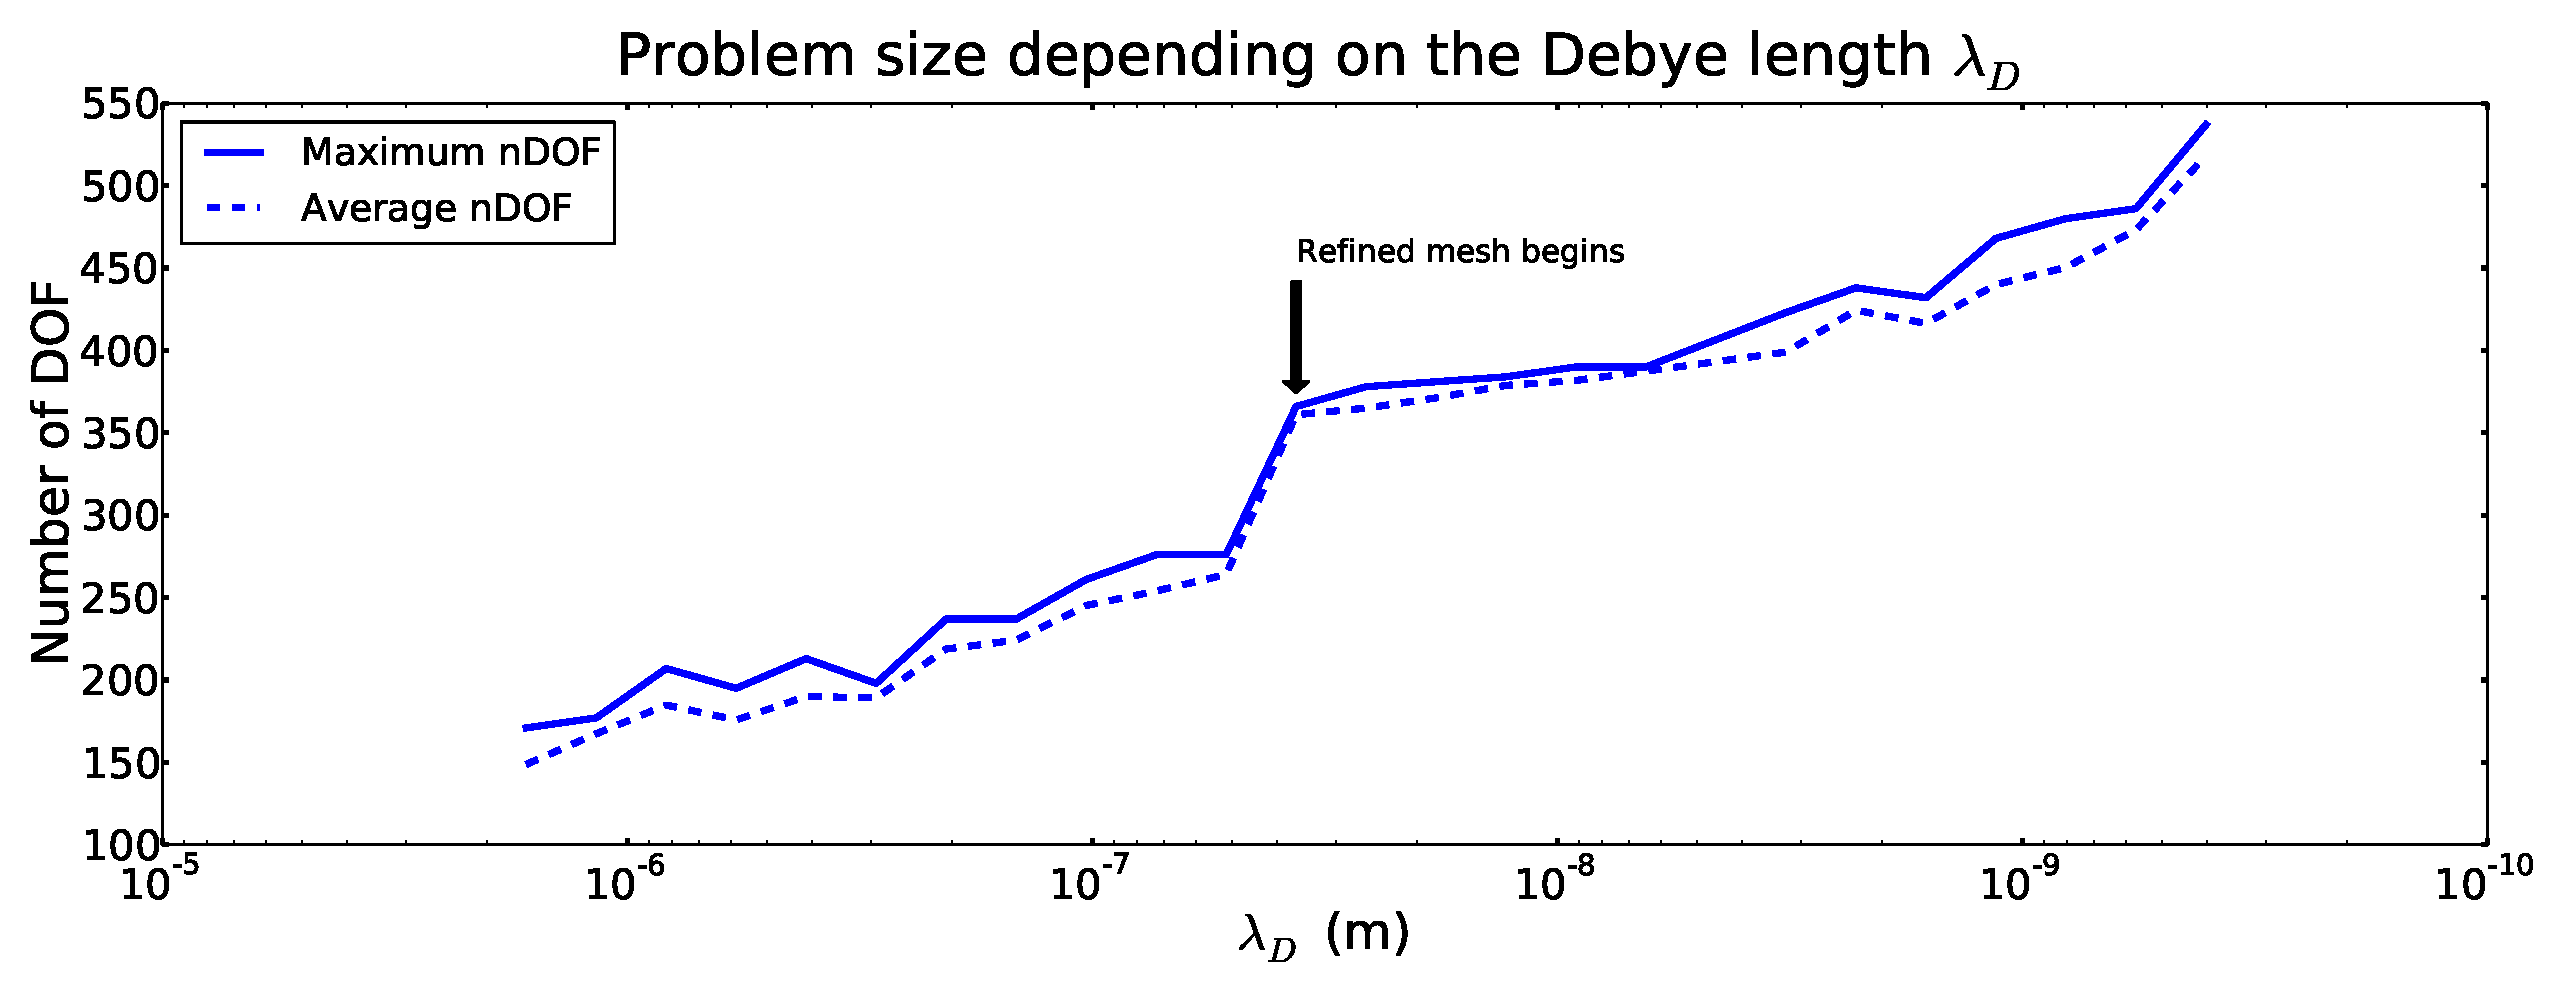
\includegraphics[width=\columnwidth]{debye_dof}
  \caption{\label{fig:debye_dof} Problem size depending on the
	Debye length. Initially the coarse mesh (shown in Fig.~\ref{fig:mesh}~(a))
	was used. It was necessary to use the fine mesh (see Fig.~\ref{fig:mesh}~(c)) 
	for smaller $\lambda_D$ values.}
  \end{centering}
\end{figure}

\begin{figure}[!ht]
  \begin{centering}
  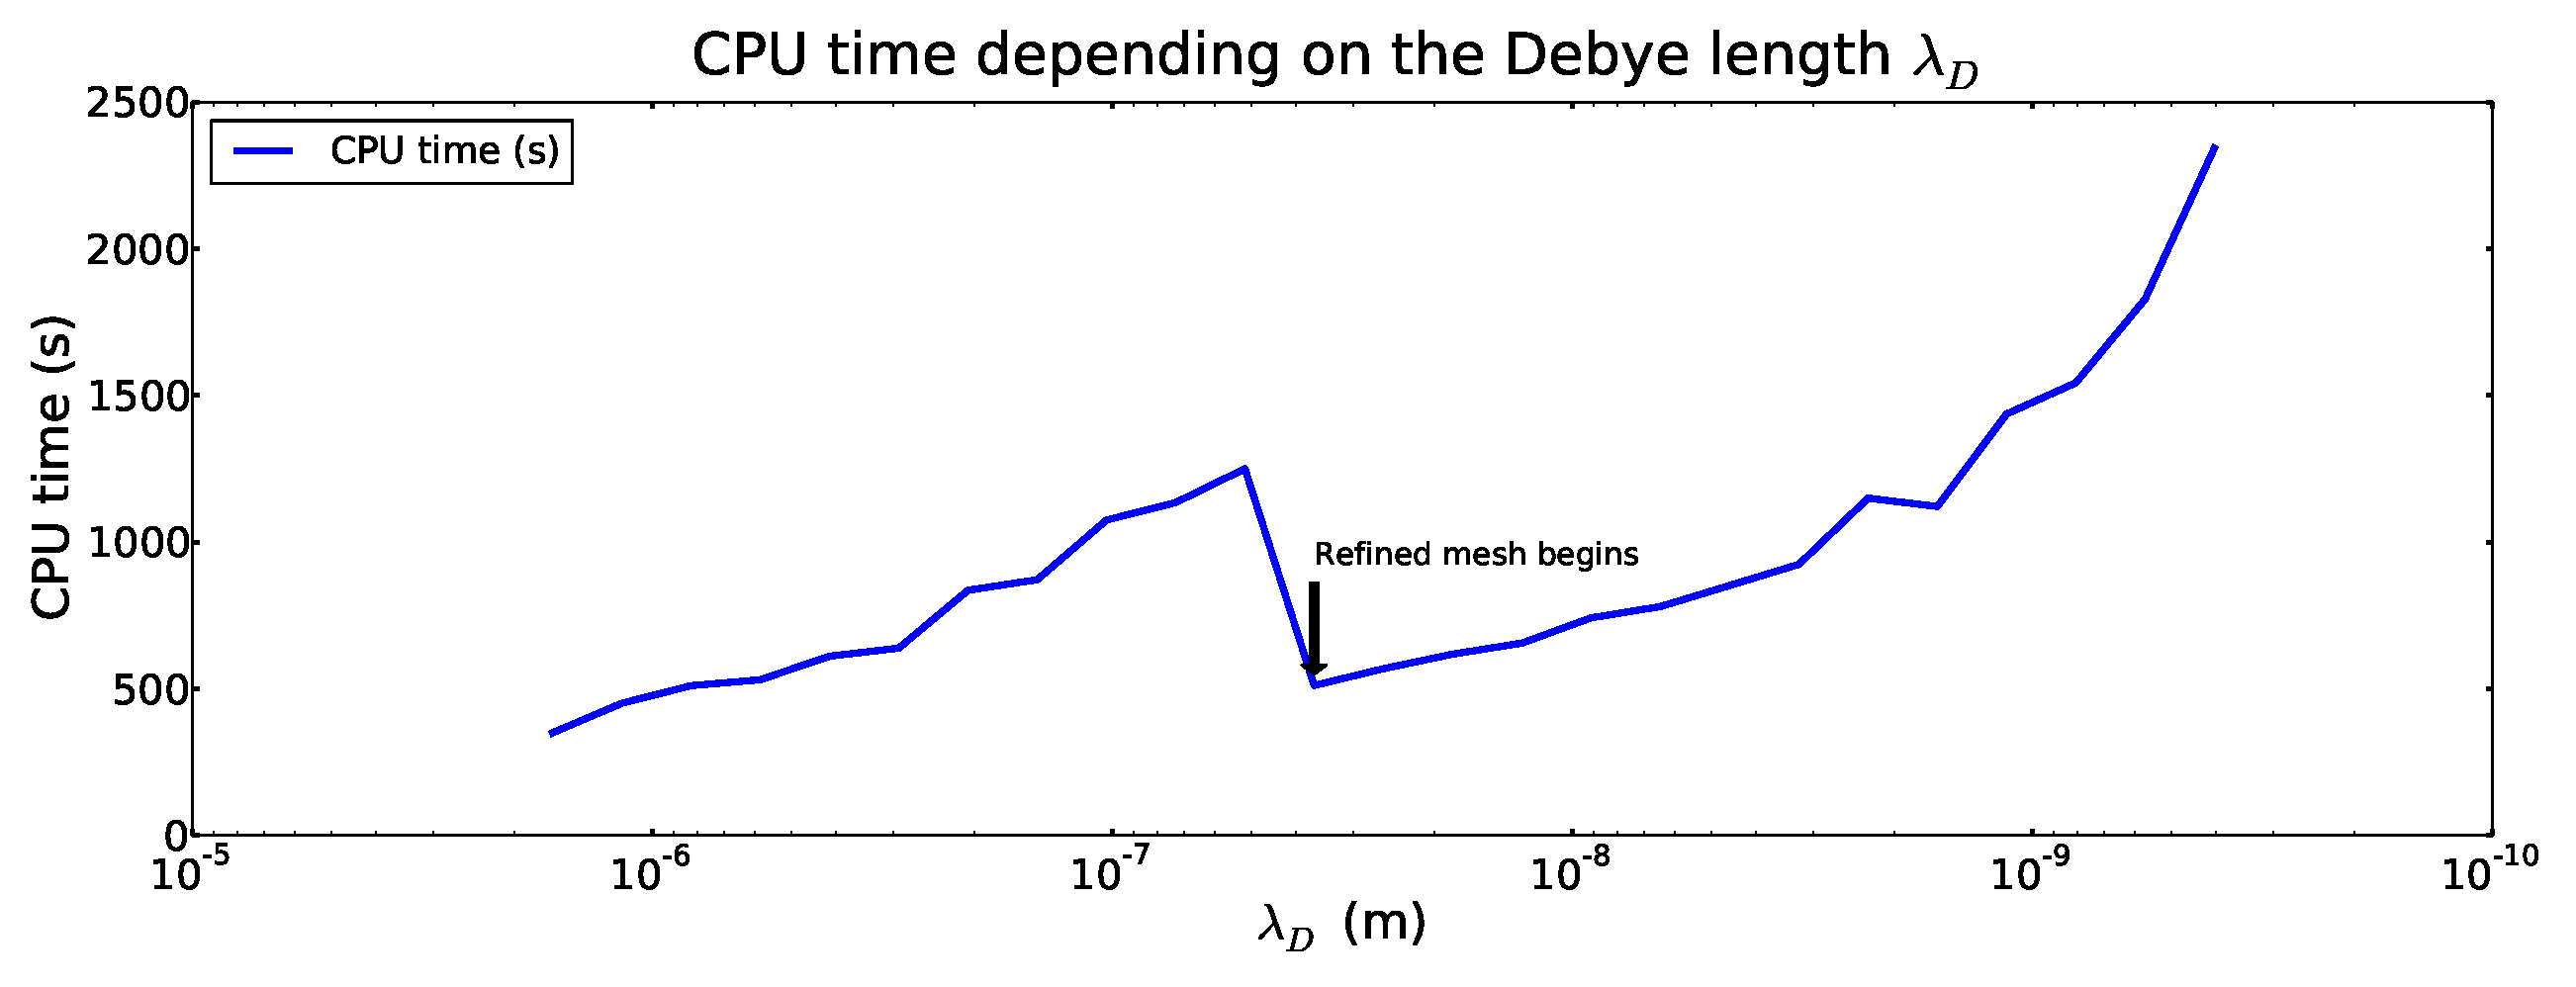
\includegraphics[width=\columnwidth]{debye_cpu}
  \caption{\label{fig:debye_cpu} CPU time depending on the
	Debye length. Initially the coarse mesh (shown in Fig.~\ref{fig:mesh}~(a))
	was used. It was necessary to use the fine mesh (see Fig.~\ref{fig:mesh}~(c)) 
	for smaller $\lambda_D$ values.}
  \end{centering}
\end{figure}
The Debye length $\lambda_D$ is the screening length in the electrolyte
solutions. Its numerical value shows the
thickness of the charged layer in the vicinity of the boundaries $\partial\Omega_1$ 
and $\partial\Omega_2$.
In all the previous simulations, the Debye screening length was determined by  the constants in
Table~\ref{Table:used-constants} and Eq.~\eqref{eq:debye}: $\lambda_D=1.7\ \mu m$. It is known that computation gets increasingly
difficult when reducing the value of $\lambda_D$.
It was our interest to see how small screening lengths can Hermes HP\_ANISO automatic
adaptivity handle. The parameter $\varepsilon$ was varied as follows:
$$\varepsilon_n=\varepsilon\times 0.5^n,$$ where $\varepsilon$ is taken from Table~\ref{Table:used-constants}. The simulations were run for each $\varepsilon_n$ and corresponding $\lambda_D$ value
and maximum number of degrees of freedom and cumulative CPU time were recorded.
The simulation time $t$ for each $\lambda_D$ was chosen to be $\tau$ --- the
characteristic time scale --- and each simulation
was divided equally into fifteen time steps. The PID controller was not used.
Fig.~\ref{fig:debye_dof} shows the maximum and average number of degrees of 
freedom during calculation
as a function of the Debye length and Fig.~\ref{fig:debye_cpu} shows cumulative CPU time as a function
of the Debye length. The simulations up to $0.52$~nm
screening length were carried out on
the initial coarse mesh. However, from $\lambda_D > 0.52$~nm, the finer initial mesh had to
be used so the existence of the large gradients of the
physical fields $c$ and $\varphi$ near the boundaries could be captured in the first place.
\begin{figure}[!ht]
  \begin{centering}
  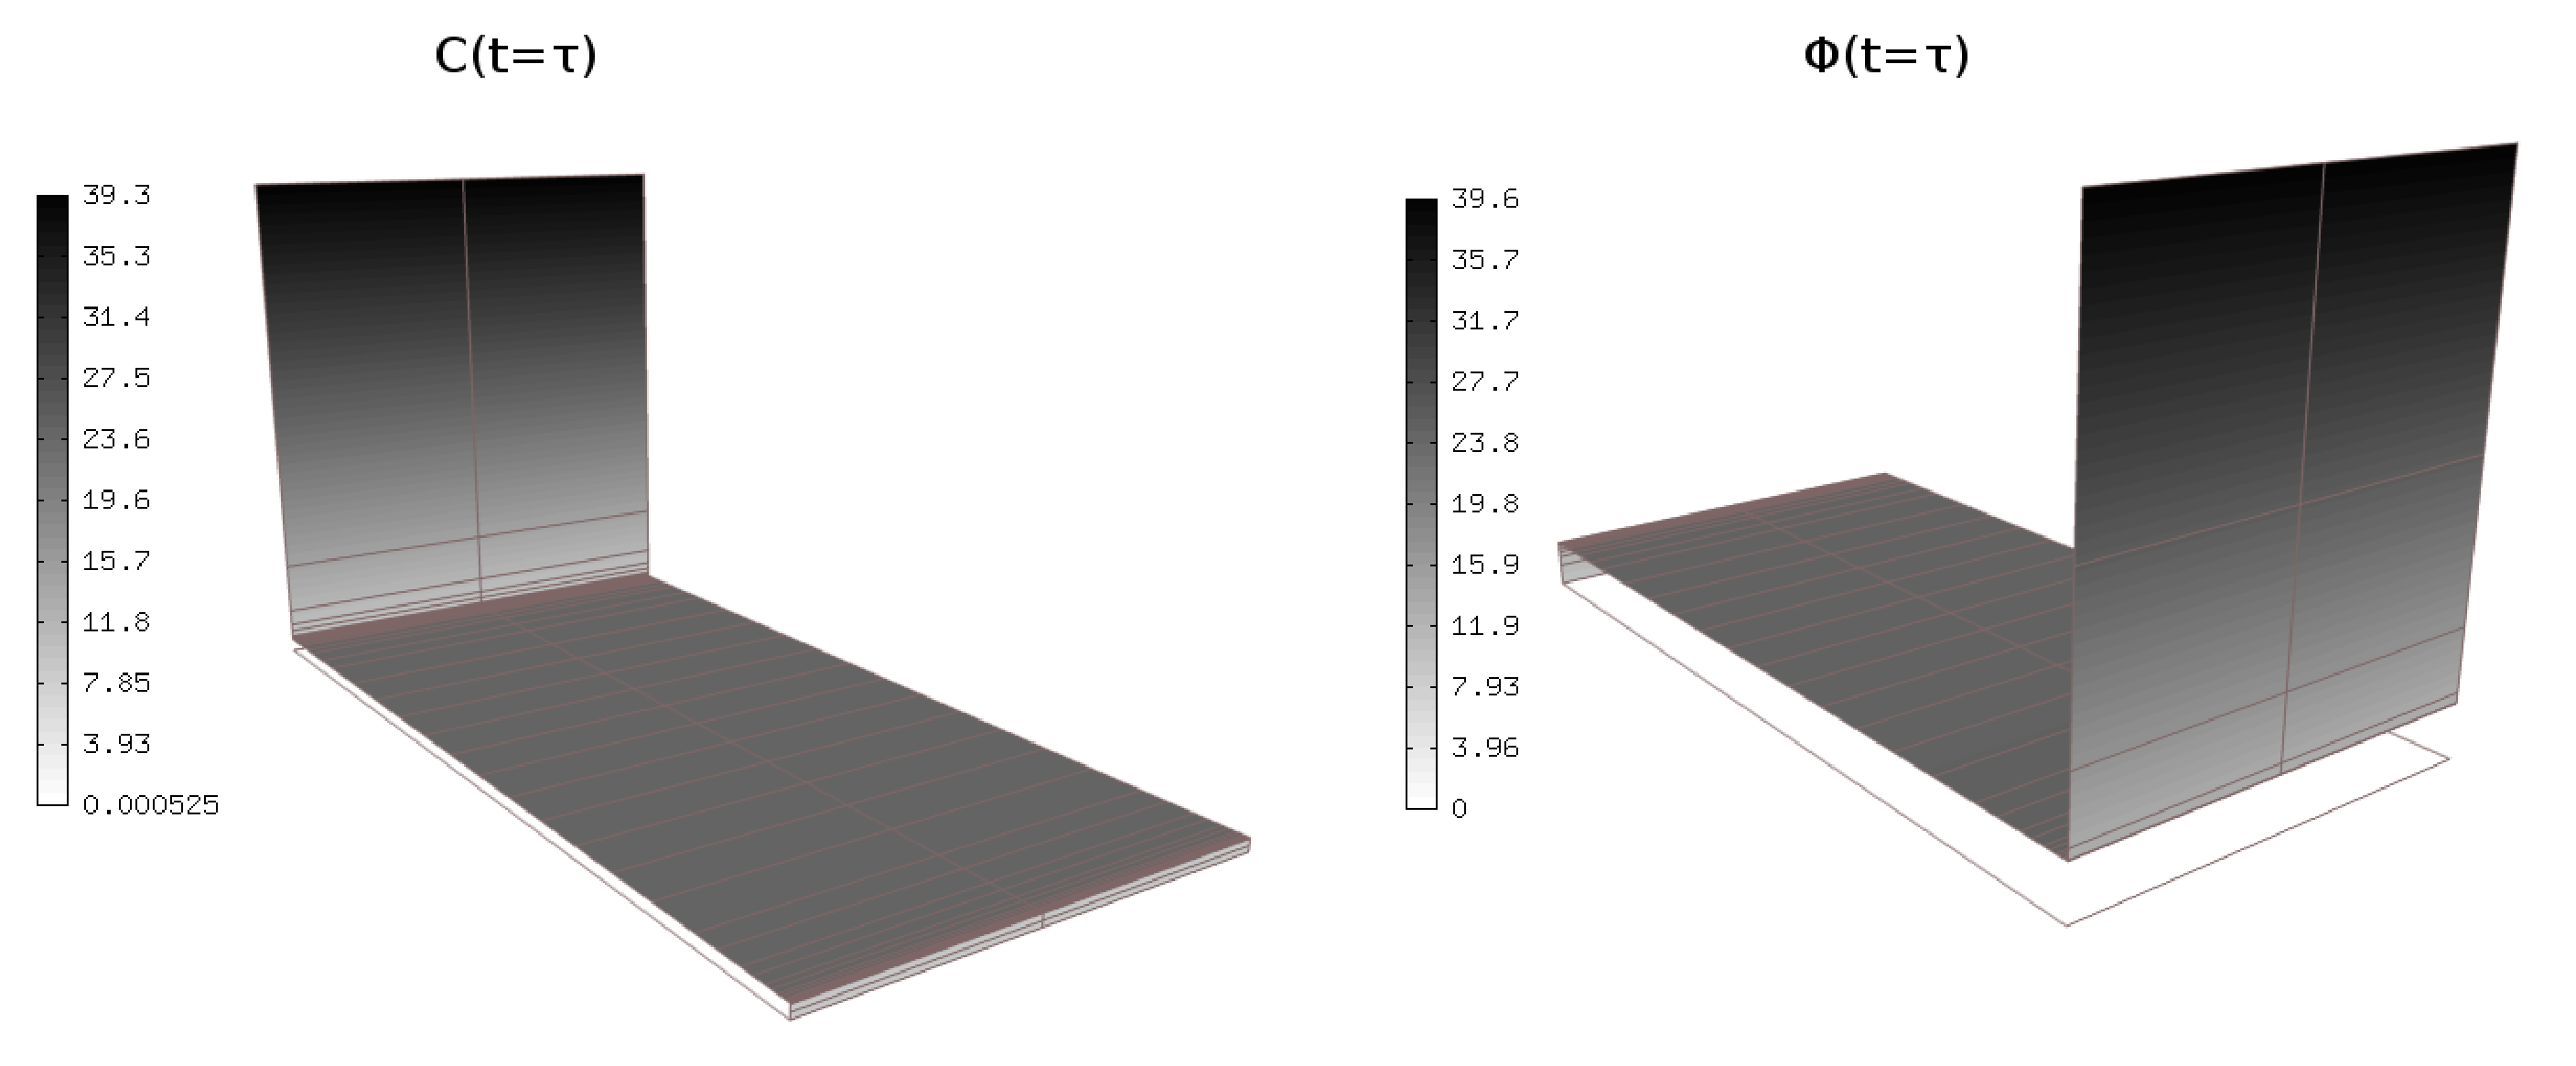
\includegraphics[width=\columnwidth]{cphitau}
  \caption{\label{fig:cphitau} Calculated fields $c$ and $\varphi$ at $t=\tau=0.81\ ms$
	for $\lambda_D=0.4\ nm$.}
  \end{centering}
\end{figure}
\noindent
The fine mesh allowed simulations with the Debye length down to $0.40$~nm. The calculated
$c$ and $\varphi$ at $t=\tau$ for $\lambda_D=0.40$~nm are shown in Fig.~\ref{fig:cphitau}.
It appears that when using even finer initial mesh and higher initial polynomial degrees, even
smaller Debye lengths could be used when necessary. The polynomial space of $c$ had
consistently higher maximum polynomial degree than that of $\varphi$, however, the difference
was less noticeable for smaller Debye lengths.

\section{Conclusion and Outlook}\label{sec:conc}

In this work the system of Nernst-Planck-Poisson equations
was solved using \emph{hp}-finite element method with adaptive
multi-mesh configuration. The weak form, residuals and
the Jacobian matrix of the system were explicitly derived
and implemented in Hermes \emph{hp}-FEM time dependent
adaptive solver.
The solution for Nernst-Planck-Poisson
problem with two field variables $C$ and $\phi$ results in 
very different field gradients in the space and time.
When using a conventional low order
FEM, finding an optimal mesh for this
type of problem such that both the error of
the solution and problem size remain small throughout the
time dependent solving process is difficult. 

In the current work we showed that using the time dependent adaptivity, 
multi-mesh configuration, and anisotropic \emph{hp} refinements, the problem
size remains very small throughout the solving process while
maintainging pre-set relative error of the solution.
Namely, Hermes refinement mode HP\_ANISO 
resulted in the smallest and fastest problem solution.
Furthermore, using the multi-mesh configuration for the variables
$C$ and $\phi$ was justified --- the adaptivity algorithm
did not refine the mesh of $\phi$ nor did increase the
polynomial degree throughout the adaptivity process. However,
the mesh was significantly refined for $C$ and also the
maximum polynomial degree was varied in the range of
$2\ldots 9$. So it is efficient to use multi-mesh in terms of
the number of degrees of freedom.

Conclusively, by using \emph{hp}-FEM with adaptive multi-mesh
configuration we can possibly reduce the problem size
of the Nernst-Planck-Poisson equation system significantly while
still maintaining prescribed precision of the solution. 
We believe, and this
is yet to be demonstrated, that this is especially
important when dealing with 3D problems in a large physical
domain with non-uniform boundary conditions.


\section*{Acknowledgments}
The second author was partially supported by the Grant Agency of the Academy of 
Sciences of the Czech Republic under Grant No. IAA100760702, and by the U.S.
Department of Energy Research Subcontract No. 00089911. 
The third author acknowledges the financial support of the U.S. Office of Naval Research 
under Award N000140910218. The fourth author acknowledges the financial support of
the Estonian Ministry of Education, grant \#SF0180008s08.

%\begin{thebibliography}{99}
%\bibitem{\ldots}..

%\end{thebibliography}
\newpage

\bibliographystyle{amsrn}    % Bibliography: Author-Date system
\bibliography{pugal-esco2010}      % pls. call your database here

\end{document}


